%%
%% Copyright 2007, 2008, 2009 Elsevier Ltd
%%
%% This file is part of the 'Elsarticle Bundle'.
%% ---------------------------------------------
%%
%% It may be distributed under the conditions of the LaTeX Project Public
%% License, either version 1.2 of this license or (at your option) any
%% later version.  The latest version of this license is in
%%    http://www.latex-project.org/lppl.txt
%% and version 1.2 or later is part of all distributions of LaTeX
%% version 1999/12/01 or later.
%%
%% The list of all files belonging to the 'Elsarticle Bundle' is
%% given in the file `manifest.txt'.
%%

%% Template article for Elsevier's document class `elsarticle'
%% with numbered style bibliographic references
%% SP 2008/03/01
%%
%%
%%
%% $Id: elsarticle-template-num.tex 4 2009-10-24 08:22:58Z rishi $
%%
%%
\documentclass[preprint,12pt]{elsarticle}

%% Use the option review to obtain double line spacing
%% \documentclass[preprint,review,12pt]{elsarticle}

%% Use the options 1p,twocolumn; 3p; 3p,twocolumn; 5p; or 5p,twocolumn
%% for a journal layout:
%% \documentclass[final,1p,times]{elsarticle}
%% \documentclass[final,1p,times,twocolumn]{elsarticle}
%% \documentclass[final,3p,times]{elsarticle}
%% \documentclass[final,3p,times,twocolumn]{elsarticle}
%% \documentclass[final,5p,times]{elsarticle}
%% \documentclass[final,5p,times,twocolumn]{elsarticle}

%% if you use PostScript figures in your article
%% use the graphics package for simple commands
%% \usepackage{graphics}
%% or use the graphicx package for more complicated commands
%% \usepackage{graphicx}
%% or use the epsfig package if you prefer to use the old commands
%% \usepackage{epsfig}

%% The amssymb package provides various useful mathematical symbols
\usepackage{amssymb}
%\usepackage{times,amsmath,amsfonts}
\usepackage{float}
\usepackage{graphicx}
\usepackage{enumerate}
\usepackage{subfigure}
\usepackage{url}
\usepackage{multirow}
\usepackage{makecell}
\usepackage{algcompatible}
\usepackage{eqparbox}
\usepackage{epsfig}
\usepackage{epstopdf}
\usepackage{mathrsfs}
\usepackage{amsmath}
\usepackage{balance}
\usepackage{algcompatible}
%% The amsthm package provides extended theorem environments
\usepackage{amsthm}

%% The lineno packages adds line numbers. Start line numbering with
%% \begin{linenumbers}, end it with \end{linenumbers}. Or switch it on
%% for the whole article with \linenumbers after \end{frontmatter}.
%% \usepackage{lineno}

%% natbib.sty is loaded by default. However, natbib options can be
%% provided with \biboptions{...} command. Following options are
%% valid:

%%   round  -  round parentheses are used (default)
%%   square -  square brackets are used   [option]
%%   curly  -  curly braces are used      {option}
%%   angle  -  angle brackets are used    <option>
%%   semicolon  -  multiple citations separated by semi-colon
%%   colon  - same as semicolon, an earlier confusion
%%   comma  -  separated by comma
%%   numbers-  selects numerical citations
%%   super  -  numerical citations as superscripts
%%   sort   -  sorts multiple citations according to order in ref. list
%%   sort&compress   -  like sort, but also compresses numerical citations
%%   compress - compresses without sorting
%%
%% \biboptions{comma,round}

% \biboptions{}

\renewcommand\algorithmiccomment[1]{%
  \hfill\#\ \eqparbox{COMMENT}{#1}%
}
\newcommand\LONGCOMMENT[1]{%
  \hfill\#\ \begin{minipage}[t]{\eqboxwidth{COMMENT}}#1\strut\end{minipage}%
}

\clubpenalty=10000
\widowpenalty=10000
\makeatletter
\newif\if@restonecol
\makeatother
\let\algorithm\relax
\let\endalgorithm\relax
\usepackage[linesnumbered,vlined,ruled]{algorithm2e}

\usepackage{xspace}
\newcommand{\qid}{\emph{qid}\xspace}
\newcommand{\qids}{\emph{qid}s\xspace}

\newcommand{\SA}{\mathcal{SA}}

\newcommand{\argmax}{\mathop{\mathrm{argmax}}}
\newcommand{\pss}{\sigma^2_{\eta_c^i}}
\newcommand{\qss}{\sigma^2_{\eta_c^j}}
\newcommand{\pww}{w^2_i}
\newcommand{\qww}{w^2_j}
\newcommand{\container}{\mathcal{C}}
\newcommand{\csize}{\kappa}
\newcommand{\linked}{\mathcal{L}}
\newcommand{\enum}{\mathcal{E}}
\newcommand{\safe}{\mathcal{S}}
\newcommand{\policy}{\mathcal{P}}
\newcommand{\natnum}{\mathbb{N}}
\newcommand{\breach}{P_\text{breach}}
\newcommand{\wrt}{w.r.t.}
\newcommand{\TRUE}{\textbf{true} }
\newcommand{\FALSE}{\textbf{false} }
\newcommand{\AND}{\textbf{and} }
\newcommand{\NOT}{\textbf{not} }
\newcommand{\RETURN}{\textbf{return} }
\newcommand{\reference}{\textbf{ref}~}
\newcommand{\shrink}{\vspace*{-3pt}}

\newcommand{\PartialSuppressor}{\textsc{PartialSuppressor} }
\newcommand{\SplitData}{\textsc{DNCSplitData} }
\newcommand{\SanitizeBuffer}{\textsc{SanitizeBuffer} }
\newcommand{\HandleLongRecord}{\textsc{HandleLong} }
\newcommand{\HandleShortRecords}{\textsc{HandleShort} }
\newcommand{\MakeRed}{\textcolor{red}}

\newcommand{\Enum}{\textsc{EnumQids} }
\newcommand{\EnumLong}{\textsc{EnumerateLong} }
\newcommand{\ClearBuffer}{\textsc{ClearBuffer} }
\newcommand{\UpdateBuffer}{\textsc{UpdateBuffer} }
\newcommand{\FindAffected}{\textsc{FindAffected} }
\newcommand{\SuppressionPolicy}{\textsc{SuppressionPolicy} }

\newcommand{\bmax}{b_\text{max}}
\newcommand{\lmin}{l_\text{min}}
\newcommand{\tmax}{t_\text{max}}
\newcommand{\dnum}{\sigma}

\newcommand{\PartialR}{\textsc{Partial(r)} }
\newcommand{\PartialL}{\textsc{Partial(l)} }
\newcommand{\PartialALL}{\textsc{Partial(all)} }

\newtheorem{theorem}{Theorem}
%\newproof{proof}{Proof}
\newtheorem{lemma}{Lemma}
\newtheorem{proposition}{Proposition}
\newtheorem{corollary}{Corollary}
\newtheorem{definition}{Definition}
\newtheorem{property}{Property}
\newtheorem{axiom}{Axiom}
\newtheorem{example}{Example}
\newcommand{\etal}{{\em et al.}\xspace}

\usepackage[usenames]{color}
\newcommand{\XH}[1]{\textcolor{blue}{[Xinhui: #1]}}
\newcommand{\KZ}[1]{\textcolor{Green}{[KZ: #1]}}

\journal{Data \& Knowledge Engineering}

\begin{document}

\begin{frontmatter}

%% Title, authors and addresses

%% use the tnoteref command within \title for footnotes;
%% use the tnotetext command for the associated footnote;
%% use the fnref command within \author or \address for footnotes;
%% use the fntext command for the associated footnote;
%% use the corref command within \author for corresponding author footnotes;
%% use the cortext command for the associated footnote;
%% use the ead command for the email address,
%% and the form \ead[url] for the home page:
%%
%% \title{Title\tnoteref{label1}}
%% \tnotetext[label1]{}
%% \author{Name\corref{cor1}\fnref{label2}}
%% \ead{email address}
%% \ead[url]{home page}
%% \fntext[label2]{}
%% \cortext[cor1]{}
%% \address{Address\fnref{label3}}
%% \fntext[label3]{}

\title{Partial Suppression of Set-Valued Data}

%% use optional labels to link authors explicitly to addresses:
%% \author[label1,label2]{<author name>}
%% \address[label1]{<address>}
%% \address[label2]{<address>}

\author{Xinhui ~Xu}
\ead{xuxinhui08@gmail.com}
\author{Xiao ~Jia}
\ead{xjia@cs.sjtu.edu.cn}
\author{Chao ~Pan}
\ead{pc660@sjtu.edu.cn}
\author{Kenny Q. ~Zhu}
\ead{kzhu@cs.sjtu.edu.cn}
\address{
Department of Computer Science \& Engineering, Shanghai Jiao Tong University,
800 Dongchuan Road, Shanghai 200240, China}

\address{}

\begin{abstract}
%% Text of abstract
Privacy-preserving set-valued data publishing is an important yet challenging
problem. In this paper, we present a novel framework for set-valued data
anonymization by partial suppression which ensures no strong inference of
sensitive information is possible regardless of the amount of background
knowledge the attacker possesses, and can be adapted to both space-time and
quality-time trade-offs as a ``pay-as-you-go'' approach.
%
While minimizing the number of item deletions, the framework attempts to
either preserve the original data distribution or retain mineable useful
association rules with limited spurious rules invented in the anonymized
data, without particular assumptions of the downstream utility of the data.
%
We also devise two novel heuristics to drive the partial suppression process
in two different directions. The first heuristic seeks to preserve the
original data distribution by minimizing the {\em Kullback-Leibler
divergence} between the original and anonymized data sets. The second
heuristic seeks to reduce the number of spurious rules when the anonymized
data is used for rule mining. Our extensive experiments show that partial
suppression significantly outperforms generalization and global suppression,
two of the existing popular anonymization techniques, in maximizing the data
utility with reasonable cost in time.
%space and time.
\end{abstract}

\begin{keyword}
%% keywords here, in the form: keyword \sep keyword

%% MSC codes here, in the form: \MSC code \sep code
%% or \MSC[2008] code \sep code (2000 is the default)

Data Anoymization \sep Partial Suppression \sep Global Suppression \sep
Generalization \sep Set-valued Data \sep Information Loss
\end{keyword}

\end{frontmatter}

%%
%% Start line numbering here if you want
%%
% \linenumbers

%% main text
%\section{}
%\label{}

%\IEEEraisesectionheading{
% %\IEEEraisesectionheading{
% %\IEEEraisesectionheading{
% \input{intro}
\section{Introduction}\label{sec:intro}
 %}
% \section{Introduction}\label{sec:intro}

% \begin{enumerate}
% \item Motivation: application scenarios (with 1-2 running examples);
% \item Characteristics of the data sources and their challenges;
% \item Briefly introduce previous approaches to extract information 
% from images including setting the document zone, and their limitations.
% \item General flow of our approach (may give a diagram here)
% \end{enumerate}
% scenary

Due to ever evolving hardware and software, many medical images
such as electro-cardio graphs (ECGs), X-ray or ultrasound images  
are directly printed and stored in hard copy formats. 
% \KZ{Insert 4 example images here.}
%Examples are shown in \figref{fig:medicalImages}. 
% These images often contain a mix of graphics and text, which
% include parameter settings of the hardware, test measurements or simple
% diagnosis. 
These images often contain a mix of graphics and text, which 
include technical settings of the hardware used, test measurements or simple diagnoses.
Recently, there has been a growing demand for digitizing such 
medical information from paper media sources, especially legacy ones, or patients who want to keep track of these documents by themselves digitally. 
Apart from scanning the graphics into a digital format, extracting 
the semi-structured textual information is also an important part of
building electronic medical records for patients. 

%\begin{figure}[!htb]
%\centering
%\subfloat[ECG]{
%\label{fig:medicalimage:ecg}
%\epsfig{file=figure/17_ori.eps, width=0.4\columnwidth}
%}
%% \hfill
%\subfloat[MRI]{
%	\label{fig:medicalimage:mrt}
%	\epsfig{file=figure/MRI.eps, width=0.4\columnwidth}
%}
%\\
%\subfloat[X-RAY]{
%\label{fig:medicalimage:xray}
%\epsfig{file=figure/X-RAY.eps, width=0.4\columnwidth}
%}
%%\hfill
%\subfloat[EEG]{
%\label{fig:medicalimage:eeg}
%\epsfig{file=figure/EEG.eps, width=0.4\columnwidth}
%}
%\caption{Examples of Medical Images}
%\label{fig:medicalImages}
%\end{figure}

Optical character recognition (OCR)  \cite{mori1992historical,smith2007overview} is 
a traditional technique used to turn images of printed text into machine encoded
text. It is well researched and performs well on plain text 
documents such as novels and reports, for a variety of languages. 
%For example, Tesseract, which is one of 
%the most popular open source multilingual recognizers, logs an error 
%rate of 3.72\% for English words and 3.77\% for simplified 
%Chinese characters\cite{smith2009adapting}. 
%Google Books \cite{googlebooks} and Gutenberg \cite{gutenberg} are
%projects which have scanned a large number of paper books into text for free and open
%access. These projects made exclusive use of OCR for this conversion and 
%achieved high accuracy \cite{vincent2007google} \cite{lebert2008project}. 
% 99\% for Gutenberg project \cite{lebert2008project}. 
% \KZ{Give the accuracy of google and gutenberg if available.}


\begin{figure}[th]
\centering
\epsfig{file=figure/17_b.eps, width=0.8\columnwidth}
\caption{An ECG image with text area (red circle) of interest.}
\label{fig:ecgexample2}
\end{figure}

For a semi-structured medical image, such as 
\figref{fig:ecgexample2}, we would like to extract the attribute-value 
pairs (e.g., {\em Vent. rate = 63 bpm}) and possibly other values such as
date ({\em 18-Nov-2010}) and time ({\em 9:13:02}) since those values endow us with lots of information about the patient. 
Existing OCR software cannot extract such structured information in a straightforward 
fashion, 
but instead it produces rather convoluted results from the whole image, 
similar to those in \figref{fig:ocrre}, which was produced by Tesseract, 
a popular multi-lingual recognizers. 
% \KZ{Maybe include the x-y coordinate info in the output as well?}  

\begin{figure}[th]
\centering
\scriptsize
\begin{verbatim}
<p class="ocr_par" title="box 263 33 444 119">
   <span class="ocr_l" title="box 264 33 336 45">
       <span class="ocrx_w" title="box 264 33 299 45">Vcnt.</span> 
       <span class="ocrx_w" title="box 308 34 336 45">rule</span> 
   </span>
   <span class='ocr_l'>
       <span class="ocrx_w" title="box 264 51 283 64">PR</span> 
       <span class="ocrx_w" title="box 291 51 346 64">Interval</span> 
       <span class="ocrx_w" title="box 389 52 411 64">140</span> 
       <span class="ocrx_w" title="box 420 55 439 64">ms</span> 
   </span>
   ...
   </span>
</p>
<p class="ocr_p" dir="ltr">
   <span class="ocr_l">
       <span class="ocrx_w" title="box 396 33 411 45">53</span> 
       <span class="ocrx_w" title="box 420 33 449 48">bpm</span> 
   </span>
</p>
\end{verbatim}
\caption{Snippet OCR results in XML, input to our framework.}
\label{fig:ocrre}
\end{figure}


%\input{xmlre1}

%However, OCR alone does not work well on semi-structured text and hence
%can't be directly used for information extraction from the aforementioned
%medical images. \KZ{Give the reason here, perhaps because OCR models are
%largely Markov based? So semi-structured data breaks the flow of text.}
%When a medical image is input to an ordinary OCR software, the spatial 
%information of the text components is often lost or mixed with noises
%and errors.
%%The reason is OCR converts the whole images into text data, in which 
%%useful information often mix with noises and errors. 
%In this paper, we would like to extract the attribute-value pairs
%and possibly other values from \figref{fig:ecgexample1} 
%and \figref{fig:ecgexample2}. 
%% or medical ultrasonography report. 
%Such images contain lots of non-textual information or noises.

% example & ref
%\begin{figure}[ht]
%\centering
%\epsfig{file=figure/46.eps, width=0.8\columnwidth}
%\caption{ECG Images From Printer1}
%\label{fig:ecgexample1}
%\end{figure}

% \begin{figure}[ht]
% \centering
% \subfloat[Printer1]{
% \label{fig:ecgexample:a}
% \epsfig{file=figure/46.eps, width=0.48\columnwidth}
% }
% \hfill
% \subfloat[Printer2]{
% \label{fig:ecgexample:b}
% \epsfig{file=figure/17.eps, width=0.48\columnwidth}
% }
% \caption{ECG images from two different printers}
% \label{fig:ecgexample}
% \end{figure}

Also, errors in the OCR text \cite{darwish2007error,taghva1996evaluation} will greatly affect the effectiveness 
of other related tasks. Much work has been done to improve the performance of the OCR\cite{kolak2003generative,cesarini1998informys}. However, there are still a number of significant challenges involved in extracting the information from medical images or OCR results in XML form. 

% First, medical images differ from pure text document in that them have 
% layout information. 
First, medical images differ from pure text documents in that 
they contain layout information.
Although most current OCR engines attempt to reproduce the physical 
layout of the text units, 
%(along with X-Y coordinates) and store them 
%in a special format such as XML 
% (\KZ{Better in the previous example})
such spatial
information is approximate and sometimes inaccurate, which is why neighboring
text blocks in \figref{fig:ecgexample2}, such as ``Vent. Rate'' and
``63 bpm'' were not automatically combined into the same XML block, but were 
rather far apart (shown in two different ``classes'') in \figref{fig:ocrre} made by OCR softwares. 
%Even for images produced by the same ECG printer, 
%the XML results can still be very different as 
The spatial layout is sensitive to many factors, such as accidental spots 
on the prints, color and contrast, or the angle of the camera. 
%In this case, solutions for other application domains, for example, the web, 
%are not well suited for information extraction from printed documents \cite{bartoli2014semisupervised}. With such inaccurate
%layout information produced by OCR,
%it is not easy to write a simple wrapper program to extract useful
%data from images, even if the images come from the same printer. 

%Writing a wrapper for each
%individual image would be tedious and counter-productive. Therefore,
%a mechanism that makes use of the spatial locality of the 
%text units in the image and 
%accommodates slight variations in the spatial layout would make the extraction
%more accurate and fault-tolerant.

%For example, \figref{fig:ocrre} is the simplified OCR results for the ECGs in 
%\figref{fig:ecgexample1} and \figref{fig:ecgexample2}. The results are in the XML format and have attritube named {\em class} 
%for layout information. Although these two images share similar format. 
%OCR engine generates different results in that it splits elements that 
%should be in the same line into two lines in the second example. 
%XML is sensitive to the layout results so it's hard to tolerate 
%all the layout results. 
%
% example check the term
% layout of ocr results can be restore, so why OCR engine don't restore the results 
% using the similar methods as we do?
% or the way we handle the layout problem is quite simple

% Delete for TIP
% Second, exiting OCR engines make heavy use of Markov properties such as n-grams
% since they primarily target the transformation of large body of text 
% \cite{kolak2003generative}. 
% % \KZ{Needs some refs here.}
% Unfortunately, the semi-structured texts in medical images are often 
% short and not even written in complete sentences, thus breaking Markov assumption. To make
% matters worse, medical images contain scientific language, which may be
% very different from the training corpora of these OCR engines.
% This explains why we see errors like ``Vcnt'' and ``rule'' 
% in \figref{fig:ocrre}. 
% %can't guarantee a perfect performance, which means 
% %there are errors and noises in the OCR results.
% %Many of them due to the fact that the data are no longer long, continous
% %sentences, thus breaking the Markov assumption made by many OCR algorithms. 
% %In \figref{fig:ocrresub:b}, ``Vent." is misrecognized as ``Vcnt.". 
% Without sufficient contextual information, OCR may also misrecognize a 
% digit as an alphabetic character, or as another similar digit. 
% Furthermore, the mix of text with images and formatting
% lines often confuses the OCR engine, which is more biased toward full
% text images.
% Exact pattern matching, as used in
% traditional information extraction, doesn't work with such noisy OCR output
% as it doesn't tolerate noises or errors in text. 
% %It's hard to autocorrect these errors 
% %because image quality is the most important affecting factor. 
% %The text we are processing can be full of no meaning words or 
% %strange numbers. 
% A fuzzy matching strategy is more desirable in this case. 
% % example, what are the traditional IEs

Second, there are many types of medical images, resulting from a variety of
medical tests. Different equipments for the same test can produce vastly 
different images. Writing individual extraction wrappers 
for the OCR outputs of all these formats is tedious and inefficient, 
and difficult for non-programmers.
%not to mention that there are significant programming barriers for 
%writing these wrappers, especially for the medical professionals who are the
%end users of these extraction results. 
%A more user-friendly approach enabling users to specify such extraction requirements would be preferred. 
%There are various kinds of medical images, such as electrocardiograph report, 
%medical ultrasonography report, etc. 
%However the basic measures for each type of medical test (e.g., ECG), 
%are very similar from machine to machine. Only the layouts are 
%different. 
% example medical images

Finally, most off-the-shelf OCR programs are pre-trained with specific 
recognition models, which may not be suitable for the extraction of 
%medical images.
%Furthermore, changes in imaging equipment technology over time may produce 
%different formats, layout, or terminology, rendering existing OCR models 
%obsolete. 
Re-training the models requires a large amount of labeled data, which may
not be available. 
%Incremental training as more labeled data arrives
%is currently not supported by any OCR product.    

%There have been some limited attempts to address some of the above challenges. 
%One solution is a plugin of an OCR program that allows the user to specify 
%target zones of interest in the image to be extracted. The zones specified for
%one image can be applied to images with slight variations by adjusting against
%a fixed reference point that is supposed to exist in all these images.
%% \KZ{I think the problem is not so much with the zones, because we also
%% have zones, but rather with the reference point.}
%% \JY{}
%% example products
%% http://www.square-9.com/automated-data-extraction-optical-character-recognition
%The problem with this solution is its high reliance on the OCR zones  
%established by the user. The performance of the results is affected by the 
%accuracy of the zones. If the zones are too big, the results will be full of 
%noise. If the zones are too small, results will miss something. 
%
%Another solution involves using the page layout analysis technique. The page layout 
%analysis technique is used to determine where the text 
%resides on a page \cite{o1993document}, 
%% \KZ{This page layout analysis approach is not clearly described. I don't understand after reading this paragraph.}
%% By using page layout analysis technique, the hierarchy of physical components 
%% can be generated and to match with the hierarchy of logical components, which 
%% is predefined. 
%this includes identifying and categorizing the 
%regions of interest in the scanned image of a text document. 
%Typically, the first step is to segment text zones from 
%non-textual zones and arrange them in their original order. 
%Then in order to analyze the logical roles of the text zones 
%(titles, captions, footnotes, etc.), logical layout analysis 
%is used for labeling the semantics of the text zones.
%Generally, page layout analysis is used for documents. The problem with applying 
%such a technique on medical images is that it creates so much noises 
%that performance is ultimately affected. 
%For medical imaging reports like ECG, useful information is often 
%found in the small components of the image, while most of the images are 
%read as noises. 
% check paper and more description, weakness, ref

%In this paper, 
%we propose a spatial data description language, which borrows its syntax from
%PADS \cite{fisher+:pads}, an ad hoc data processing language, 
%for describing semi-structured data in medical images. 
%% ref
%We call this language OCR description language, or ODL. 
%ODL is designed for extracting and parsing semi-structured text data 
%from images. We believe that  information extraction from those data in ODL form may be much easier than extracting information from rough data or data in XML form, which means that our preprocessing part proves to be necessary.
%%An example ODL description for the image in 
%%\figref{fig:ecgexample2} is shown in 
%%\figref{fig:description}. \KZ{Make this description two column, and give
%%some brief explanation of this description here.} 
%%The parsing result of this description is shown
%%in \figref{fig:parsing result}. \KZ{Give some explanation of the results,
%%otherwise don't show the result here. E.g., you need to explain what F, E, etc.
%%mean. You want to say that even though rate has been recognized as rule,
%%the bpm value was still extracted (but still wrong!).}
%% \KZ{I removed the preprocessing part, cos it's not important. Talk about it in
%% discussion sec.}
%%The our approach starts by preprocessing the images for text results.
%To use this framework, the user first describes the components in the image
%that he or she is interested in extracting. This includes constant strings
%and variables of different data types.   
%ODL allows the user to specify the approximate spatial layout and constraints on
%the data, e.g., integers within 
%a certain range, real numbers with certain decimal points, etc. 
%%This information is then as the key component in our fuzzy matching strategy. 
%The system then automatically generates a parser for these medical images.
%This parser uses the output XML from OCR with spatial information as an input, 
%and outputs a data structure with values extracted for each variables
%in the description, unless there is an unrecoverable error during the parsing process.
%In addition, approximate layout information and constraints are used in parsing process 
%to tolerate noises and small format variations in the input images. 
%%Specifically, this method could be called fuzzy matching, meaning that more candidates could be saved after the parsing process.  It's obvious that we may have a higher probability to obtain the accurate result if more candidates are kept so that fuzzy match should be used properly in our system.
%%An autogenerated parser based on the ODL description can release us from 
%%repetitive work. In this way, we turn the task of writing complex parsers 
%%into describing information on images.
%
%
%When users process many images of the same format, the system 
%automatically discovers parsing errors given the current model and 
%prompts the user to manually correct some of the frequent and prominent
%errors, which effectively serves as an online labeling function. 
%These incrementally labeled data are then used to update the parsing model. 


%It should be emphasized that the incremental learning model is very important in our whole system. Incremental learning is a machine learning paradigm where the learning process takes place whenever we have new examples or data added to our baisc data set, leading to a most striking difference between incremental learning and traditional machine learning: it does not assume the availability of a sufficient training set before the learning process. What incremental learning in our system is really impressive: it does not require a relatively good and stable training set at first time. In fact, it could improve the parsing result with even relatively rough training sets at first by absorbing new data or corrective information as time passes in dynamic systems. Besides, the process would be very effective when there are some new images coming in since training process would not learn from scratch, which might waste time and computation resource.

%At last, we propose an incrementally human correction framwork which can 
%make the best use of human correction to handle the misrecognition problem. 
% Base on our experiments on about 500 real life ECG images, 
% our approach achieves p1 and p2 after p3 times human correction. 
% experimental results

% \begin{figure}[h]
% \begin{lstlisting}
% Oenum str_month_t{
% 	"Jan", "Feb", "Mar", "Apr",
% 	"May", "Jun", "Jul", "Aug",
% 	"Sept", "Oct", "Nov", "Dec"
% };

% Ounion month_t{
% 	Oint(1,12)	num;
% 	str_month_t	str;
% };

% Ostruct time_t{
% 	Oint(1,31)	day;
% 	"-";
% 	month_t	month;
% 	"-";
% 	Oint	year;
% };

% Ostruct triple_t{
% 	"Vent.";
% 	hskip(\s)	skip1;
% 	"rate";
% 	Oint x;
% 	"bpm";
% 	vskip(\n)	skip2;
% };

% Oscource Ostruct entry_t{
% 	time_t(<-,-,-,0.3l>) t;
% 	triple_t(<0.1w,-,0.5w,->) d;
% };
% \end{lstlisting}
% \caption{Description}\label{fig:description}
% \end{figure}


In order to solve above problems, We design a system which makes three main contributions:
\begin{enumerate}
\item Based on some previous work on data description language \cite{lamport1986document,taft1999post,fisher+:pads},we design a new declarative spatial data description language called \textit{OCR description language}, or ODL,
which allows users to specify spatial and data constraints in medical 
images(\secref{sec:syntax});
\item We propose a noise-tolerant parser which takes OCR results
the ODL description as input and outputs a data structure with values 
extracted for each variables in the description (\secref{sec:semantics});
\item We propose an incremental manual correction 
framework\cite{von2008recaptcha,zhu2012learnpads++}, which 
takes advantage of user corrections  and improves the productivity
significantly (\secref{sec:correction}).
%To be more specific, the framework improves the traditional machine learning methods by using a incremental learning process to avoid starting from scratch when we are trying to apply human corrections in the system. That means the framework would be more effective than most corrective systems.
\end{enumerate}


\section{Introduction}\label{sec:intro}
 %}
% \section{Introduction}\label{sec:intro}

% \begin{enumerate}
% \item Motivation: application scenarios (with 1-2 running examples);
% \item Characteristics of the data sources and their challenges;
% \item Briefly introduce previous approaches to extract information 
% from images including setting the document zone, and their limitations.
% \item General flow of our approach (may give a diagram here)
% \end{enumerate}
% scenary

Due to ever evolving hardware and software, many medical images
such as electro-cardio graphs (ECGs), X-ray or ultrasound images  
are directly printed and stored in hard copy formats. 
% \KZ{Insert 4 example images here.}
%Examples are shown in \figref{fig:medicalImages}. 
% These images often contain a mix of graphics and text, which
% include parameter settings of the hardware, test measurements or simple
% diagnosis. 
These images often contain a mix of graphics and text, which 
include technical settings of the hardware used, test measurements or simple diagnoses.
Recently, there has been a growing demand for digitizing such 
medical information from paper media sources, especially legacy ones, or patients who want to keep track of these documents by themselves digitally. 
Apart from scanning the graphics into a digital format, extracting 
the semi-structured textual information is also an important part of
building electronic medical records for patients. 

%\begin{figure}[!htb]
%\centering
%\subfloat[ECG]{
%\label{fig:medicalimage:ecg}
%\epsfig{file=figure/17_ori.eps, width=0.4\columnwidth}
%}
%% \hfill
%\subfloat[MRI]{
%	\label{fig:medicalimage:mrt}
%	\epsfig{file=figure/MRI.eps, width=0.4\columnwidth}
%}
%\\
%\subfloat[X-RAY]{
%\label{fig:medicalimage:xray}
%\epsfig{file=figure/X-RAY.eps, width=0.4\columnwidth}
%}
%%\hfill
%\subfloat[EEG]{
%\label{fig:medicalimage:eeg}
%\epsfig{file=figure/EEG.eps, width=0.4\columnwidth}
%}
%\caption{Examples of Medical Images}
%\label{fig:medicalImages}
%\end{figure}

Optical character recognition (OCR)  \cite{mori1992historical,smith2007overview} is 
a traditional technique used to turn images of printed text into machine encoded
text. It is well researched and performs well on plain text 
documents such as novels and reports, for a variety of languages. 
%For example, Tesseract, which is one of 
%the most popular open source multilingual recognizers, logs an error 
%rate of 3.72\% for English words and 3.77\% for simplified 
%Chinese characters\cite{smith2009adapting}. 
%Google Books \cite{googlebooks} and Gutenberg \cite{gutenberg} are
%projects which have scanned a large number of paper books into text for free and open
%access. These projects made exclusive use of OCR for this conversion and 
%achieved high accuracy \cite{vincent2007google} \cite{lebert2008project}. 
% 99\% for Gutenberg project \cite{lebert2008project}. 
% \KZ{Give the accuracy of google and gutenberg if available.}


\begin{figure}[th]
\centering
\epsfig{file=figure/17_b.eps, width=0.8\columnwidth}
\caption{An ECG image with text area (red circle) of interest.}
\label{fig:ecgexample2}
\end{figure}

For a semi-structured medical image, such as 
\figref{fig:ecgexample2}, we would like to extract the attribute-value 
pairs (e.g., {\em Vent. rate = 63 bpm}) and possibly other values such as
date ({\em 18-Nov-2010}) and time ({\em 9:13:02}) since those values endow us with lots of information about the patient. 
Existing OCR software cannot extract such structured information in a straightforward 
fashion, 
but instead it produces rather convoluted results from the whole image, 
similar to those in \figref{fig:ocrre}, which was produced by Tesseract, 
a popular multi-lingual recognizers. 
% \KZ{Maybe include the x-y coordinate info in the output as well?}  

\begin{figure}[th]
\centering
\scriptsize
\begin{verbatim}
<p class="ocr_par" title="box 263 33 444 119">
   <span class="ocr_l" title="box 264 33 336 45">
       <span class="ocrx_w" title="box 264 33 299 45">Vcnt.</span> 
       <span class="ocrx_w" title="box 308 34 336 45">rule</span> 
   </span>
   <span class='ocr_l'>
       <span class="ocrx_w" title="box 264 51 283 64">PR</span> 
       <span class="ocrx_w" title="box 291 51 346 64">Interval</span> 
       <span class="ocrx_w" title="box 389 52 411 64">140</span> 
       <span class="ocrx_w" title="box 420 55 439 64">ms</span> 
   </span>
   ...
   </span>
</p>
<p class="ocr_p" dir="ltr">
   <span class="ocr_l">
       <span class="ocrx_w" title="box 396 33 411 45">53</span> 
       <span class="ocrx_w" title="box 420 33 449 48">bpm</span> 
   </span>
</p>
\end{verbatim}
\caption{Snippet OCR results in XML, input to our framework.}
\label{fig:ocrre}
\end{figure}


%% \begin{figure}[ht]
% \centering
% \subfigure[]{
% \label{fig:subfig:a}
% \begin{minipage}[b]{0.2\textwidth}
%\newsavebox{\firstlisting}
%\begin{lrbox}{\firstlisting}% Store first listing
%\begin{lstlisting}
%<p class='ocr_par' dir='ltr'>
%   <span class='ocr_line' id='line_2'>
%       <span class='ocrx_word' id='word_6'>Vent.</span>
%       <span class='ocrx_word' id='word_7'>rate</span>
%       <span class='ocrx_word' id='word_8'>65</span>
%       <span class='ocrx_word' id='word_9'>bpm</span>
%   </span>
%   <span class='ocr_line' id='line_3'>
%       <span class='ocrx_word' id='word_14'>PR</span>
%       <span class='ocrx_word' id='word_15'>interval</span>
%       <span class='ocrx_word' id='word_16'>162</span>
%       <span class='ocrx_word' id='word_17'>ms</span>
%   </span>
%    ...
%</p>
%\end{lstlisting}
%\end{lrbox}
% \end{minipage}
% }
% \hspace[1in]
% \subfigure[]{
% % \label{fig:subfig:b}
% % \begin{minipage}[b]{0.2\textwidth}
\newsavebox{\secondlisting}
\begin{lrbox}{\secondlisting}
% \tiny
\begin{lstlisting}[basicstyle=\tiny,]
<p class="ocr_par" title="box 263 33 444 119">
   <span class="ocr_l" title="box 264 33 336 45">
       <span class="ocrx_w" title="box 264 33 299 45">Vcnt.</span>
       <span class="ocrx_w" title="box 308 34 336 45">rule</span>
   </span>
   <span class='ocr_l'>
       <span class="ocrx_w" title="box 264 51 283 64">PR</span>
       <span class="ocrx_w" title="box 291 51 346 64">Interval</span>
       <span class="ocrx_w" title="box 389 52 411 64">140</span>
       <span class="ocrx_w" title="box 420 55 439 64">ms</span>
   </span>
   ...
   </span>
</p>
<p class="ocr_p" dir="ltr">
   <span class="ocr_l">
       <span class="ocrx_w" title="box 396 33 411 45">53</span>
       <span class="ocrx_w" title="box 420 33 449 48">bpm</span>
   </span>
</p>
\end{lstlisting}
\end{lrbox}
% % \end{minipage}
% }

% \KZ{\figref{fig:ocrre} is output from what software? Tesseract?}
\begin{figure*}[th]
%\subfloat[Image From Printer1]{
%\label{fig:ocrresub:a}
%\scalebox{0.8}{\usebox{\firstlisting}}}
%\hfill
%\subfloat[Image From Printer2]{
\scalebox{1.6}{\usebox{\secondlisting}}
% \label{fig:ocrre}
\caption{A fragment of raw OCR results for ECG with layout information.}
%\caption{Simplified OCR Results in XML for an ECG with Layout Information}
%\label{fig:ocrresub:b}
\label{fig:running-xml}
\end{figure*}

% \lipsum[2]


%However, OCR alone does not work well on semi-structured text and hence
%can't be directly used for information extraction from the aforementioned
%medical images. \KZ{Give the reason here, perhaps because OCR models are
%largely Markov based? So semi-structured data breaks the flow of text.}
%When a medical image is input to an ordinary OCR software, the spatial 
%information of the text components is often lost or mixed with noises
%and errors.
%%The reason is OCR converts the whole images into text data, in which 
%%useful information often mix with noises and errors. 
%In this paper, we would like to extract the attribute-value pairs
%and possibly other values from \figref{fig:ecgexample1} 
%and \figref{fig:ecgexample2}. 
%% or medical ultrasonography report. 
%Such images contain lots of non-textual information or noises.

% example & ref
%\begin{figure}[ht]
%\centering
%\epsfig{file=figure/46.eps, width=0.8\columnwidth}
%\caption{ECG Images From Printer1}
%\label{fig:ecgexample1}
%\end{figure}

% \begin{figure}[ht]
% \centering
% \subfloat[Printer1]{
% \label{fig:ecgexample:a}
% \epsfig{file=figure/46.eps, width=0.48\columnwidth}
% }
% \hfill
% \subfloat[Printer2]{
% \label{fig:ecgexample:b}
% \epsfig{file=figure/17.eps, width=0.48\columnwidth}
% }
% \caption{ECG images from two different printers}
% \label{fig:ecgexample}
% \end{figure}

Also, errors in the OCR text \cite{darwish2007error,taghva1996evaluation} will greatly affect the effectiveness 
of other related tasks. Much work has been done to improve the performance of the OCR\cite{kolak2003generative,cesarini1998informys}. However, there are still a number of significant challenges involved in extracting the information from medical images or OCR results in XML form. 

% First, medical images differ from pure text document in that them have 
% layout information. 
First, medical images differ from pure text documents in that 
they contain layout information.
Although most current OCR engines attempt to reproduce the physical 
layout of the text units, 
%(along with X-Y coordinates) and store them 
%in a special format such as XML 
% (\KZ{Better in the previous example})
such spatial
information is approximate and sometimes inaccurate, which is why neighboring
text blocks in \figref{fig:ecgexample2}, such as ``Vent. Rate'' and
``63 bpm'' were not automatically combined into the same XML block, but were 
rather far apart (shown in two different ``classes'') in \figref{fig:ocrre} made by OCR softwares. 
%Even for images produced by the same ECG printer, 
%the XML results can still be very different as 
The spatial layout is sensitive to many factors, such as accidental spots 
on the prints, color and contrast, or the angle of the camera. 
%In this case, solutions for other application domains, for example, the web, 
%are not well suited for information extraction from printed documents \cite{bartoli2014semisupervised}. With such inaccurate
%layout information produced by OCR,
%it is not easy to write a simple wrapper program to extract useful
%data from images, even if the images come from the same printer. 

%Writing a wrapper for each
%individual image would be tedious and counter-productive. Therefore,
%a mechanism that makes use of the spatial locality of the 
%text units in the image and 
%accommodates slight variations in the spatial layout would make the extraction
%more accurate and fault-tolerant.

%For example, \figref{fig:ocrre} is the simplified OCR results for the ECGs in 
%\figref{fig:ecgexample1} and \figref{fig:ecgexample2}. The results are in the XML format and have attritube named {\em class} 
%for layout information. Although these two images share similar format. 
%OCR engine generates different results in that it splits elements that 
%should be in the same line into two lines in the second example. 
%XML is sensitive to the layout results so it's hard to tolerate 
%all the layout results. 
%
% example check the term
% layout of ocr results can be restore, so why OCR engine don't restore the results 
% using the similar methods as we do?
% or the way we handle the layout problem is quite simple

% Delete for TIP
% Second, exiting OCR engines make heavy use of Markov properties such as n-grams
% since they primarily target the transformation of large body of text 
% \cite{kolak2003generative}. 
% % \KZ{Needs some refs here.}
% Unfortunately, the semi-structured texts in medical images are often 
% short and not even written in complete sentences, thus breaking Markov assumption. To make
% matters worse, medical images contain scientific language, which may be
% very different from the training corpora of these OCR engines.
% This explains why we see errors like ``Vcnt'' and ``rule'' 
% in \figref{fig:ocrre}. 
% %can't guarantee a perfect performance, which means 
% %there are errors and noises in the OCR results.
% %Many of them due to the fact that the data are no longer long, continous
% %sentences, thus breaking the Markov assumption made by many OCR algorithms. 
% %In \figref{fig:ocrresub:b}, ``Vent." is misrecognized as ``Vcnt.". 
% Without sufficient contextual information, OCR may also misrecognize a 
% digit as an alphabetic character, or as another similar digit. 
% Furthermore, the mix of text with images and formatting
% lines often confuses the OCR engine, which is more biased toward full
% text images.
% Exact pattern matching, as used in
% traditional information extraction, doesn't work with such noisy OCR output
% as it doesn't tolerate noises or errors in text. 
% %It's hard to autocorrect these errors 
% %because image quality is the most important affecting factor. 
% %The text we are processing can be full of no meaning words or 
% %strange numbers. 
% A fuzzy matching strategy is more desirable in this case. 
% % example, what are the traditional IEs

Second, there are many types of medical images, resulting from a variety of
medical tests. Different equipments for the same test can produce vastly 
different images. Writing individual extraction wrappers 
for the OCR outputs of all these formats is tedious and inefficient, 
and difficult for non-programmers.
%not to mention that there are significant programming barriers for 
%writing these wrappers, especially for the medical professionals who are the
%end users of these extraction results. 
%A more user-friendly approach enabling users to specify such extraction requirements would be preferred. 
%There are various kinds of medical images, such as electrocardiograph report, 
%medical ultrasonography report, etc. 
%However the basic measures for each type of medical test (e.g., ECG), 
%are very similar from machine to machine. Only the layouts are 
%different. 
% example medical images

Finally, most off-the-shelf OCR programs are pre-trained with specific 
recognition models, which may not be suitable for the extraction of 
%medical images.
%Furthermore, changes in imaging equipment technology over time may produce 
%different formats, layout, or terminology, rendering existing OCR models 
%obsolete. 
Re-training the models requires a large amount of labeled data, which may
not be available. 
%Incremental training as more labeled data arrives
%is currently not supported by any OCR product.    

%There have been some limited attempts to address some of the above challenges. 
%One solution is a plugin of an OCR program that allows the user to specify 
%target zones of interest in the image to be extracted. The zones specified for
%one image can be applied to images with slight variations by adjusting against
%a fixed reference point that is supposed to exist in all these images.
%% \KZ{I think the problem is not so much with the zones, because we also
%% have zones, but rather with the reference point.}
%% \JY{}
%% example products
%% http://www.square-9.com/automated-data-extraction-optical-character-recognition
%The problem with this solution is its high reliance on the OCR zones  
%established by the user. The performance of the results is affected by the 
%accuracy of the zones. If the zones are too big, the results will be full of 
%noise. If the zones are too small, results will miss something. 
%
%Another solution involves using the page layout analysis technique. The page layout 
%analysis technique is used to determine where the text 
%resides on a page \cite{o1993document}, 
%% \KZ{This page layout analysis approach is not clearly described. I don't understand after reading this paragraph.}
%% By using page layout analysis technique, the hierarchy of physical components 
%% can be generated and to match with the hierarchy of logical components, which 
%% is predefined. 
%this includes identifying and categorizing the 
%regions of interest in the scanned image of a text document. 
%Typically, the first step is to segment text zones from 
%non-textual zones and arrange them in their original order. 
%Then in order to analyze the logical roles of the text zones 
%(titles, captions, footnotes, etc.), logical layout analysis 
%is used for labeling the semantics of the text zones.
%Generally, page layout analysis is used for documents. The problem with applying 
%such a technique on medical images is that it creates so much noises 
%that performance is ultimately affected. 
%For medical imaging reports like ECG, useful information is often 
%found in the small components of the image, while most of the images are 
%read as noises. 
% check paper and more description, weakness, ref

%In this paper, 
%we propose a spatial data description language, which borrows its syntax from
%PADS \cite{fisher+:pads}, an ad hoc data processing language, 
%for describing semi-structured data in medical images. 
%% ref
%We call this language OCR description language, or ODL. 
%ODL is designed for extracting and parsing semi-structured text data 
%from images. We believe that  information extraction from those data in ODL form may be much easier than extracting information from rough data or data in XML form, which means that our preprocessing part proves to be necessary.
%%An example ODL description for the image in 
%%\figref{fig:ecgexample2} is shown in 
%%\figref{fig:description}. \KZ{Make this description two column, and give
%%some brief explanation of this description here.} 
%%The parsing result of this description is shown
%%in \figref{fig:parsing result}. \KZ{Give some explanation of the results,
%%otherwise don't show the result here. E.g., you need to explain what F, E, etc.
%%mean. You want to say that even though rate has been recognized as rule,
%%the bpm value was still extracted (but still wrong!).}
%% \KZ{I removed the preprocessing part, cos it's not important. Talk about it in
%% discussion sec.}
%%The our approach starts by preprocessing the images for text results.
%To use this framework, the user first describes the components in the image
%that he or she is interested in extracting. This includes constant strings
%and variables of different data types.   
%ODL allows the user to specify the approximate spatial layout and constraints on
%the data, e.g., integers within 
%a certain range, real numbers with certain decimal points, etc. 
%%This information is then as the key component in our fuzzy matching strategy. 
%The system then automatically generates a parser for these medical images.
%This parser uses the output XML from OCR with spatial information as an input, 
%and outputs a data structure with values extracted for each variables
%in the description, unless there is an unrecoverable error during the parsing process.
%In addition, approximate layout information and constraints are used in parsing process 
%to tolerate noises and small format variations in the input images. 
%%Specifically, this method could be called fuzzy matching, meaning that more candidates could be saved after the parsing process.  It's obvious that we may have a higher probability to obtain the accurate result if more candidates are kept so that fuzzy match should be used properly in our system.
%%An autogenerated parser based on the ODL description can release us from 
%%repetitive work. In this way, we turn the task of writing complex parsers 
%%into describing information on images.
%
%
%When users process many images of the same format, the system 
%automatically discovers parsing errors given the current model and 
%prompts the user to manually correct some of the frequent and prominent
%errors, which effectively serves as an online labeling function. 
%These incrementally labeled data are then used to update the parsing model. 


%It should be emphasized that the incremental learning model is very important in our whole system. Incremental learning is a machine learning paradigm where the learning process takes place whenever we have new examples or data added to our baisc data set, leading to a most striking difference between incremental learning and traditional machine learning: it does not assume the availability of a sufficient training set before the learning process. What incremental learning in our system is really impressive: it does not require a relatively good and stable training set at first time. In fact, it could improve the parsing result with even relatively rough training sets at first by absorbing new data or corrective information as time passes in dynamic systems. Besides, the process would be very effective when there are some new images coming in since training process would not learn from scratch, which might waste time and computation resource.

%At last, we propose an incrementally human correction framwork which can 
%make the best use of human correction to handle the misrecognition problem. 
% Base on our experiments on about 500 real life ECG images, 
% our approach achieves p1 and p2 after p3 times human correction. 
% experimental results

% \begin{figure}[h]
% \begin{lstlisting}
% Oenum str_month_t{
% 	"Jan", "Feb", "Mar", "Apr",
% 	"May", "Jun", "Jul", "Aug",
% 	"Sept", "Oct", "Nov", "Dec"
% };

% Ounion month_t{
% 	Oint(1,12)	num;
% 	str_month_t	str;
% };

% Ostruct time_t{
% 	Oint(1,31)	day;
% 	"-";
% 	month_t	month;
% 	"-";
% 	Oint	year;
% };

% Ostruct triple_t{
% 	"Vent.";
% 	hskip(\s)	skip1;
% 	"rate";
% 	Oint x;
% 	"bpm";
% 	vskip(\n)	skip2;
% };

% Oscource Ostruct entry_t{
% 	time_t(<-,-,-,0.3l>) t;
% 	triple_t(<0.1w,-,0.5w,->) d;
% };
% \end{lstlisting}
% \caption{Description}\label{fig:description}
% \end{figure}


In order to solve above problems, We design a system which makes three main contributions:
\begin{enumerate}
\item Based on some previous work on data description language \cite{lamport1986document,taft1999post,fisher+:pads},we design a new declarative spatial data description language called \textit{OCR description language}, or ODL,
which allows users to specify spatial and data constraints in medical 
images(\secref{sec:syntax});
\item We propose a noise-tolerant parser which takes OCR results
the ODL description as input and outputs a data structure with values 
extracted for each variables in the description (\secref{sec:semantics});
\item We propose an incremental manual correction 
framework\cite{von2008recaptcha,zhu2012learnpads++}, which 
takes advantage of user corrections  and improves the productivity
significantly (\secref{sec:correction}).
%To be more specific, the framework improves the traditional machine learning methods by using a incremental learning process to avoid starting from scratch when we are trying to apply human corrections in the system. That means the framework would be more effective than most corrective systems.
\end{enumerate}


\section{Introduction}\label{sec:intro}
 %}
% \section{Introduction}\label{sec:intro}

% \begin{enumerate}
% \item Motivation: application scenarios (with 1-2 running examples);
% \item Characteristics of the data sources and their challenges;
% \item Briefly introduce previous approaches to extract information 
% from images including setting the document zone, and their limitations.
% \item General flow of our approach (may give a diagram here)
% \end{enumerate}
% scenary

Due to ever evolving hardware and software, many medical images
such as electro-cardio graphs (ECGs), X-ray or ultrasound images  
are directly printed and stored in hard copy formats. 
% \KZ{Insert 4 example images here.}
%Examples are shown in \figref{fig:medicalImages}. 
% These images often contain a mix of graphics and text, which
% include parameter settings of the hardware, test measurements or simple
% diagnosis. 
These images often contain a mix of graphics and text, which 
include technical settings of the hardware used, test measurements or simple diagnoses.
Recently, there has been a growing demand for digitizing such 
medical information from paper media sources, especially legacy ones, or patients who want to keep track of these documents by themselves digitally. 
Apart from scanning the graphics into a digital format, extracting 
the semi-structured textual information is also an important part of
building electronic medical records for patients. 

%\begin{figure}[!htb]
%\centering
%\subfloat[ECG]{
%\label{fig:medicalimage:ecg}
%\epsfig{file=figure/17_ori.eps, width=0.4\columnwidth}
%}
%% \hfill
%\subfloat[MRI]{
%	\label{fig:medicalimage:mrt}
%	\epsfig{file=figure/MRI.eps, width=0.4\columnwidth}
%}
%\\
%\subfloat[X-RAY]{
%\label{fig:medicalimage:xray}
%\epsfig{file=figure/X-RAY.eps, width=0.4\columnwidth}
%}
%%\hfill
%\subfloat[EEG]{
%\label{fig:medicalimage:eeg}
%\epsfig{file=figure/EEG.eps, width=0.4\columnwidth}
%}
%\caption{Examples of Medical Images}
%\label{fig:medicalImages}
%\end{figure}

Optical character recognition (OCR)  \cite{mori1992historical,smith2007overview} is 
a traditional technique used to turn images of printed text into machine encoded
text. It is well researched and performs well on plain text 
documents such as novels and reports, for a variety of languages. 
%For example, Tesseract, which is one of 
%the most popular open source multilingual recognizers, logs an error 
%rate of 3.72\% for English words and 3.77\% for simplified 
%Chinese characters\cite{smith2009adapting}. 
%Google Books \cite{googlebooks} and Gutenberg \cite{gutenberg} are
%projects which have scanned a large number of paper books into text for free and open
%access. These projects made exclusive use of OCR for this conversion and 
%achieved high accuracy \cite{vincent2007google} \cite{lebert2008project}. 
% 99\% for Gutenberg project \cite{lebert2008project}. 
% \KZ{Give the accuracy of google and gutenberg if available.}


\begin{figure}[th]
\centering
\epsfig{file=figure/17_b.eps, width=0.8\columnwidth}
\caption{An ECG image with text area (red circle) of interest.}
\label{fig:ecgexample2}
\end{figure}

For a semi-structured medical image, such as 
\figref{fig:ecgexample2}, we would like to extract the attribute-value 
pairs (e.g., {\em Vent. rate = 63 bpm}) and possibly other values such as
date ({\em 18-Nov-2010}) and time ({\em 9:13:02}) since those values endow us with lots of information about the patient. 
Existing OCR software cannot extract such structured information in a straightforward 
fashion, 
but instead it produces rather convoluted results from the whole image, 
similar to those in \figref{fig:ocrre}, which was produced by Tesseract, 
a popular multi-lingual recognizers. 
% \KZ{Maybe include the x-y coordinate info in the output as well?}  

\begin{figure}[th]
\centering
\scriptsize
\begin{verbatim}
<p class="ocr_par" title="box 263 33 444 119">
   <span class="ocr_l" title="box 264 33 336 45">
       <span class="ocrx_w" title="box 264 33 299 45">Vcnt.</span> 
       <span class="ocrx_w" title="box 308 34 336 45">rule</span> 
   </span>
   <span class='ocr_l'>
       <span class="ocrx_w" title="box 264 51 283 64">PR</span> 
       <span class="ocrx_w" title="box 291 51 346 64">Interval</span> 
       <span class="ocrx_w" title="box 389 52 411 64">140</span> 
       <span class="ocrx_w" title="box 420 55 439 64">ms</span> 
   </span>
   ...
   </span>
</p>
<p class="ocr_p" dir="ltr">
   <span class="ocr_l">
       <span class="ocrx_w" title="box 396 33 411 45">53</span> 
       <span class="ocrx_w" title="box 420 33 449 48">bpm</span> 
   </span>
</p>
\end{verbatim}
\caption{Snippet OCR results in XML, input to our framework.}
\label{fig:ocrre}
\end{figure}


%% \begin{figure}[ht]
% \centering
% \subfigure[]{
% \label{fig:subfig:a}
% \begin{minipage}[b]{0.2\textwidth}
%\newsavebox{\firstlisting}
%\begin{lrbox}{\firstlisting}% Store first listing
%\begin{lstlisting}
%<p class='ocr_par' dir='ltr'>
%   <span class='ocr_line' id='line_2'>
%       <span class='ocrx_word' id='word_6'>Vent.</span>
%       <span class='ocrx_word' id='word_7'>rate</span>
%       <span class='ocrx_word' id='word_8'>65</span>
%       <span class='ocrx_word' id='word_9'>bpm</span>
%   </span>
%   <span class='ocr_line' id='line_3'>
%       <span class='ocrx_word' id='word_14'>PR</span>
%       <span class='ocrx_word' id='word_15'>interval</span>
%       <span class='ocrx_word' id='word_16'>162</span>
%       <span class='ocrx_word' id='word_17'>ms</span>
%   </span>
%    ...
%</p>
%\end{lstlisting}
%\end{lrbox}
% \end{minipage}
% }
% \hspace[1in]
% \subfigure[]{
% % \label{fig:subfig:b}
% % \begin{minipage}[b]{0.2\textwidth}
\newsavebox{\secondlisting}
\begin{lrbox}{\secondlisting}
% \tiny
\begin{lstlisting}[basicstyle=\tiny,]
<p class="ocr_par" title="box 263 33 444 119">
   <span class="ocr_l" title="box 264 33 336 45">
       <span class="ocrx_w" title="box 264 33 299 45">Vcnt.</span>
       <span class="ocrx_w" title="box 308 34 336 45">rule</span>
   </span>
   <span class='ocr_l'>
       <span class="ocrx_w" title="box 264 51 283 64">PR</span>
       <span class="ocrx_w" title="box 291 51 346 64">Interval</span>
       <span class="ocrx_w" title="box 389 52 411 64">140</span>
       <span class="ocrx_w" title="box 420 55 439 64">ms</span>
   </span>
   ...
   </span>
</p>
<p class="ocr_p" dir="ltr">
   <span class="ocr_l">
       <span class="ocrx_w" title="box 396 33 411 45">53</span>
       <span class="ocrx_w" title="box 420 33 449 48">bpm</span>
   </span>
</p>
\end{lstlisting}
\end{lrbox}
% % \end{minipage}
% }

% \KZ{\figref{fig:ocrre} is output from what software? Tesseract?}
\begin{figure*}[th]
%\subfloat[Image From Printer1]{
%\label{fig:ocrresub:a}
%\scalebox{0.8}{\usebox{\firstlisting}}}
%\hfill
%\subfloat[Image From Printer2]{
\scalebox{1.6}{\usebox{\secondlisting}}
% \label{fig:ocrre}
\caption{A fragment of raw OCR results for ECG with layout information.}
%\caption{Simplified OCR Results in XML for an ECG with Layout Information}
%\label{fig:ocrresub:b}
\label{fig:running-xml}
\end{figure*}

% \lipsum[2]


%However, OCR alone does not work well on semi-structured text and hence
%can't be directly used for information extraction from the aforementioned
%medical images. \KZ{Give the reason here, perhaps because OCR models are
%largely Markov based? So semi-structured data breaks the flow of text.}
%When a medical image is input to an ordinary OCR software, the spatial 
%information of the text components is often lost or mixed with noises
%and errors.
%%The reason is OCR converts the whole images into text data, in which 
%%useful information often mix with noises and errors. 
%In this paper, we would like to extract the attribute-value pairs
%and possibly other values from \figref{fig:ecgexample1} 
%and \figref{fig:ecgexample2}. 
%% or medical ultrasonography report. 
%Such images contain lots of non-textual information or noises.

% example & ref
%\begin{figure}[ht]
%\centering
%\epsfig{file=figure/46.eps, width=0.8\columnwidth}
%\caption{ECG Images From Printer1}
%\label{fig:ecgexample1}
%\end{figure}

% \begin{figure}[ht]
% \centering
% \subfloat[Printer1]{
% \label{fig:ecgexample:a}
% \epsfig{file=figure/46.eps, width=0.48\columnwidth}
% }
% \hfill
% \subfloat[Printer2]{
% \label{fig:ecgexample:b}
% \epsfig{file=figure/17.eps, width=0.48\columnwidth}
% }
% \caption{ECG images from two different printers}
% \label{fig:ecgexample}
% \end{figure}

Also, errors in the OCR text \cite{darwish2007error,taghva1996evaluation} will greatly affect the effectiveness 
of other related tasks. Much work has been done to improve the performance of the OCR\cite{kolak2003generative,cesarini1998informys}. However, there are still a number of significant challenges involved in extracting the information from medical images or OCR results in XML form. 

% First, medical images differ from pure text document in that them have 
% layout information. 
First, medical images differ from pure text documents in that 
they contain layout information.
Although most current OCR engines attempt to reproduce the physical 
layout of the text units, 
%(along with X-Y coordinates) and store them 
%in a special format such as XML 
% (\KZ{Better in the previous example})
such spatial
information is approximate and sometimes inaccurate, which is why neighboring
text blocks in \figref{fig:ecgexample2}, such as ``Vent. Rate'' and
``63 bpm'' were not automatically combined into the same XML block, but were 
rather far apart (shown in two different ``classes'') in \figref{fig:ocrre} made by OCR softwares. 
%Even for images produced by the same ECG printer, 
%the XML results can still be very different as 
The spatial layout is sensitive to many factors, such as accidental spots 
on the prints, color and contrast, or the angle of the camera. 
%In this case, solutions for other application domains, for example, the web, 
%are not well suited for information extraction from printed documents \cite{bartoli2014semisupervised}. With such inaccurate
%layout information produced by OCR,
%it is not easy to write a simple wrapper program to extract useful
%data from images, even if the images come from the same printer. 

%Writing a wrapper for each
%individual image would be tedious and counter-productive. Therefore,
%a mechanism that makes use of the spatial locality of the 
%text units in the image and 
%accommodates slight variations in the spatial layout would make the extraction
%more accurate and fault-tolerant.

%For example, \figref{fig:ocrre} is the simplified OCR results for the ECGs in 
%\figref{fig:ecgexample1} and \figref{fig:ecgexample2}. The results are in the XML format and have attritube named {\em class} 
%for layout information. Although these two images share similar format. 
%OCR engine generates different results in that it splits elements that 
%should be in the same line into two lines in the second example. 
%XML is sensitive to the layout results so it's hard to tolerate 
%all the layout results. 
%
% example check the term
% layout of ocr results can be restore, so why OCR engine don't restore the results 
% using the similar methods as we do?
% or the way we handle the layout problem is quite simple

% Delete for TIP
% Second, exiting OCR engines make heavy use of Markov properties such as n-grams
% since they primarily target the transformation of large body of text 
% \cite{kolak2003generative}. 
% % \KZ{Needs some refs here.}
% Unfortunately, the semi-structured texts in medical images are often 
% short and not even written in complete sentences, thus breaking Markov assumption. To make
% matters worse, medical images contain scientific language, which may be
% very different from the training corpora of these OCR engines.
% This explains why we see errors like ``Vcnt'' and ``rule'' 
% in \figref{fig:ocrre}. 
% %can't guarantee a perfect performance, which means 
% %there are errors and noises in the OCR results.
% %Many of them due to the fact that the data are no longer long, continous
% %sentences, thus breaking the Markov assumption made by many OCR algorithms. 
% %In \figref{fig:ocrresub:b}, ``Vent." is misrecognized as ``Vcnt.". 
% Without sufficient contextual information, OCR may also misrecognize a 
% digit as an alphabetic character, or as another similar digit. 
% Furthermore, the mix of text with images and formatting
% lines often confuses the OCR engine, which is more biased toward full
% text images.
% Exact pattern matching, as used in
% traditional information extraction, doesn't work with such noisy OCR output
% as it doesn't tolerate noises or errors in text. 
% %It's hard to autocorrect these errors 
% %because image quality is the most important affecting factor. 
% %The text we are processing can be full of no meaning words or 
% %strange numbers. 
% A fuzzy matching strategy is more desirable in this case. 
% % example, what are the traditional IEs

Second, there are many types of medical images, resulting from a variety of
medical tests. Different equipments for the same test can produce vastly 
different images. Writing individual extraction wrappers 
for the OCR outputs of all these formats is tedious and inefficient, 
and difficult for non-programmers.
%not to mention that there are significant programming barriers for 
%writing these wrappers, especially for the medical professionals who are the
%end users of these extraction results. 
%A more user-friendly approach enabling users to specify such extraction requirements would be preferred. 
%There are various kinds of medical images, such as electrocardiograph report, 
%medical ultrasonography report, etc. 
%However the basic measures for each type of medical test (e.g., ECG), 
%are very similar from machine to machine. Only the layouts are 
%different. 
% example medical images

Finally, most off-the-shelf OCR programs are pre-trained with specific 
recognition models, which may not be suitable for the extraction of 
%medical images.
%Furthermore, changes in imaging equipment technology over time may produce 
%different formats, layout, or terminology, rendering existing OCR models 
%obsolete. 
Re-training the models requires a large amount of labeled data, which may
not be available. 
%Incremental training as more labeled data arrives
%is currently not supported by any OCR product.    

%There have been some limited attempts to address some of the above challenges. 
%One solution is a plugin of an OCR program that allows the user to specify 
%target zones of interest in the image to be extracted. The zones specified for
%one image can be applied to images with slight variations by adjusting against
%a fixed reference point that is supposed to exist in all these images.
%% \KZ{I think the problem is not so much with the zones, because we also
%% have zones, but rather with the reference point.}
%% \JY{}
%% example products
%% http://www.square-9.com/automated-data-extraction-optical-character-recognition
%The problem with this solution is its high reliance on the OCR zones  
%established by the user. The performance of the results is affected by the 
%accuracy of the zones. If the zones are too big, the results will be full of 
%noise. If the zones are too small, results will miss something. 
%
%Another solution involves using the page layout analysis technique. The page layout 
%analysis technique is used to determine where the text 
%resides on a page \cite{o1993document}, 
%% \KZ{This page layout analysis approach is not clearly described. I don't understand after reading this paragraph.}
%% By using page layout analysis technique, the hierarchy of physical components 
%% can be generated and to match with the hierarchy of logical components, which 
%% is predefined. 
%this includes identifying and categorizing the 
%regions of interest in the scanned image of a text document. 
%Typically, the first step is to segment text zones from 
%non-textual zones and arrange them in their original order. 
%Then in order to analyze the logical roles of the text zones 
%(titles, captions, footnotes, etc.), logical layout analysis 
%is used for labeling the semantics of the text zones.
%Generally, page layout analysis is used for documents. The problem with applying 
%such a technique on medical images is that it creates so much noises 
%that performance is ultimately affected. 
%For medical imaging reports like ECG, useful information is often 
%found in the small components of the image, while most of the images are 
%read as noises. 
% check paper and more description, weakness, ref

%In this paper, 
%we propose a spatial data description language, which borrows its syntax from
%PADS \cite{fisher+:pads}, an ad hoc data processing language, 
%for describing semi-structured data in medical images. 
%% ref
%We call this language OCR description language, or ODL. 
%ODL is designed for extracting and parsing semi-structured text data 
%from images. We believe that  information extraction from those data in ODL form may be much easier than extracting information from rough data or data in XML form, which means that our preprocessing part proves to be necessary.
%%An example ODL description for the image in 
%%\figref{fig:ecgexample2} is shown in 
%%\figref{fig:description}. \KZ{Make this description two column, and give
%%some brief explanation of this description here.} 
%%The parsing result of this description is shown
%%in \figref{fig:parsing result}. \KZ{Give some explanation of the results,
%%otherwise don't show the result here. E.g., you need to explain what F, E, etc.
%%mean. You want to say that even though rate has been recognized as rule,
%%the bpm value was still extracted (but still wrong!).}
%% \KZ{I removed the preprocessing part, cos it's not important. Talk about it in
%% discussion sec.}
%%The our approach starts by preprocessing the images for text results.
%To use this framework, the user first describes the components in the image
%that he or she is interested in extracting. This includes constant strings
%and variables of different data types.   
%ODL allows the user to specify the approximate spatial layout and constraints on
%the data, e.g., integers within 
%a certain range, real numbers with certain decimal points, etc. 
%%This information is then as the key component in our fuzzy matching strategy. 
%The system then automatically generates a parser for these medical images.
%This parser uses the output XML from OCR with spatial information as an input, 
%and outputs a data structure with values extracted for each variables
%in the description, unless there is an unrecoverable error during the parsing process.
%In addition, approximate layout information and constraints are used in parsing process 
%to tolerate noises and small format variations in the input images. 
%%Specifically, this method could be called fuzzy matching, meaning that more candidates could be saved after the parsing process.  It's obvious that we may have a higher probability to obtain the accurate result if more candidates are kept so that fuzzy match should be used properly in our system.
%%An autogenerated parser based on the ODL description can release us from 
%%repetitive work. In this way, we turn the task of writing complex parsers 
%%into describing information on images.
%
%
%When users process many images of the same format, the system 
%automatically discovers parsing errors given the current model and 
%prompts the user to manually correct some of the frequent and prominent
%errors, which effectively serves as an online labeling function. 
%These incrementally labeled data are then used to update the parsing model. 


%It should be emphasized that the incremental learning model is very important in our whole system. Incremental learning is a machine learning paradigm where the learning process takes place whenever we have new examples or data added to our baisc data set, leading to a most striking difference between incremental learning and traditional machine learning: it does not assume the availability of a sufficient training set before the learning process. What incremental learning in our system is really impressive: it does not require a relatively good and stable training set at first time. In fact, it could improve the parsing result with even relatively rough training sets at first by absorbing new data or corrective information as time passes in dynamic systems. Besides, the process would be very effective when there are some new images coming in since training process would not learn from scratch, which might waste time and computation resource.

%At last, we propose an incrementally human correction framwork which can 
%make the best use of human correction to handle the misrecognition problem. 
% Base on our experiments on about 500 real life ECG images, 
% our approach achieves p1 and p2 after p3 times human correction. 
% experimental results

% \begin{figure}[h]
% \begin{lstlisting}
% Oenum str_month_t{
% 	"Jan", "Feb", "Mar", "Apr",
% 	"May", "Jun", "Jul", "Aug",
% 	"Sept", "Oct", "Nov", "Dec"
% };

% Ounion month_t{
% 	Oint(1,12)	num;
% 	str_month_t	str;
% };

% Ostruct time_t{
% 	Oint(1,31)	day;
% 	"-";
% 	month_t	month;
% 	"-";
% 	Oint	year;
% };

% Ostruct triple_t{
% 	"Vent.";
% 	hskip(\s)	skip1;
% 	"rate";
% 	Oint x;
% 	"bpm";
% 	vskip(\n)	skip2;
% };

% Oscource Ostruct entry_t{
% 	time_t(<-,-,-,0.3l>) t;
% 	triple_t(<0.1w,-,0.5w,->) d;
% };
% \end{lstlisting}
% \caption{Description}\label{fig:description}
% \end{figure}


In order to solve above problems, We design a system which makes three main contributions:
\begin{enumerate}
\item Based on some previous work on data description language \cite{lamport1986document,taft1999post,fisher+:pads},we design a new declarative spatial data description language called \textit{OCR description language}, or ODL,
which allows users to specify spatial and data constraints in medical 
images(\secref{sec:syntax});
\item We propose a noise-tolerant parser which takes OCR results
the ODL description as input and outputs a data structure with values 
extracted for each variables in the description (\secref{sec:semantics});
\item We propose an incremental manual correction 
framework\cite{von2008recaptcha,zhu2012learnpads++}, which 
takes advantage of user corrections  and improves the productivity
significantly (\secref{sec:correction}).
%To be more specific, the framework improves the traditional machine learning methods by using a incremental learning process to avoid starting from scratch when we are trying to apply human corrections in the system. That means the framework would be more effective than most corrective systems.
\end{enumerate}


\section{Problem Definition}
\label{sec:prob}

In this section, the problem of partial suppression is formally described,
and before which, some preliminary mathematical concepts are defined as
follows.

%\subsection{Notations and Definitions}
%A {\em multiset} $S$ is a set which allows repetitive elements, while the
%{\em power multiset} $\mathbb{N}^S$ is the set of all subsets of the multiset
%$S$.
%Examples or formal definitions of these are given below.
%\begin{description}
%  \item[Multiset] $[a,a,b]$ is the same as $(\{a,b\},\{(a,2),(b,1)\})$
%  \item[Power set] $2^S$ is the power set of the set $S$
%  \item[Power multiset] $\mathbb{N}^S$ is the power multiset of the set $S$
%\end{description}

A {\em multiset} is a set which allows repetitive elements, while a {\em
power set} is the set of all subsets of a set. Examples or formal definitions
of these are given below.
\begin{description}
  \item[Multiset] \hspace{2em} $[a,a,b]$ is the same as
      $(\{a,b\},\{(a,2),(b,1)\})$
  \item[Power set]  \hspace{2em}  $2^S$ is the power set of the set $S$
  \item[Power multiset] \hspace{4em} $\mathbb{N}^S$ is the power multiset
      of the set $S$
\end{description}

\begin{table}[th]
\centering
\caption{Notations for Problem Definition}
\label{table:problem_notations}
\begin{tabular}{m{0.28\columnwidth}|m{0.6\columnwidth}}
  \hline
  \textbf{Symbol} & \textbf{Definition} \\
  \hline
  $D = D_S \cup D_N$ & the domain, which is the set of all possible items \\ \hline
  $D_S$ & the sensitive domain \\ \hline
  $D_N$ & the non-sensitive domain \\ \hline
  $T\in\natnum^{2^D}$ & a set-valued table, which is a multiset of $m$ transaction records \\ \hline
  $T[i]\in T$ & the $i$-th record of $T$ \\ \hline
  $R\in T$ & a transaction record %, which is a set of items drawn from $D$
  \\ \hline
  $|R|$ & the number of items contained in $R$ \\ \hline
  $I$ & an itemset, which is a subset of $D$\\ \hline
  $q$ & a \emph{quasi-identifier} (also \qid), which is a set of items (\textbf{sensitive items also allowed}) taken from any record in table $T$ \\ \hline
  $\enum(R) = 2^R - \{\emptyset\}$ & the \qid enumeration of $R$, which is the power set of $R$ except the $\emptyset$ \\ \hline
  $\displaystyle Q(T)=\bigcup_{R\in T} \enum(R)$ & the set of all \qids in table $T$ \\ \hline
  $\rho$ & the strong inference/association rule threshold \\ \hline
  $\mathcal{A}(q,e)$ & an inference/association rule $q\rightarrow e$\\  \hline
  $\SA(q,e)$ & a sensitive association rule $\mathcal{A}(q,e)$  if $e$ contains at least one sensitive item\\  \hline
  $sup_{T}(I)$ & the support of $I$ is the number of transactions $t\in T$ such that $I\subset t$\\ \hline
  $conf_{T}(q,e)$& the confidence of inference $\mathcal{A}(q,e)$ is $\frac{sup_T(q\cup e)}{sup_T(q)}$\\ \hline
\end{tabular}
\end{table}
%A set-valued table $T$ is a multiset of transaction records,
%  each record $R \in T$ is a set of items drawn from domain $D$.
%  $D$ is the union of two non-intersecting set, sensitive domain $D_S$ and non-sensitive domain $D_N$.
%We follow the step of \cite{Sweeney2002:k-anonymity} and
%  extend the definition \emph{quasi-identifier} ($qid$) in relational database for set-valued data.
%Then we give a series of other definitions related with $qid$.
%As simple as you can imagine, a $qid$ is just a set of items taken from $D$.
%$Q$ is a set of $qid$s, $\Omega(R_i)$ is the $qid$ enumeration of $R$ which is the power set of $R$ except the $\emptyset$.
%The column count $cc$ of row $R$ is the number of items contained in $R$.
Table \ref{table:problem_notations} lists the detailed notations used in the
rest of this paper. Next we define a number of important notations before
presenting the problem definition.

\begin{definition}[Container]
The \emph{container} of an itemset $I$ in table $T$ is defined as \[
\container_T(I) = \{ i \in \natnum : I \subseteq T[i], 1 \leq i \leq |T| \}
.\]
\end{definition}

\begin{definition}[Linked Items]
All sensitive items linked by a \qid $q$ in table $T$ is defined as \[
\linked_T(q) = \{ e \in D_S-q : sup_{T}(q\cup\{e\}) > 0 \} .\]
\end{definition}
 According to the definition, $sup_{T}(I)$=$|\container_T(I)|$.
 Also we will use $\container(I)$, $\linked(q)$, $sup(I)$,
$conf(q,e)$ to represent $\container_T(I)$, $\linked_T(q)$, $sup_{T}(I)$ and
$conf_{T}(q,e)$ respectively when $T$ is the only table within discussion.

\subsection{Privacy Model}
We reuse the $\rho$-uncertainty privacy model
proposed by Cao \etal \cite{Cao:2010:rho} which requires that the confidence of any sensitive
association rules is not above $\rho$. Next we formalize the
privacy requirement.
%Let $T$ be a set-valued table and the domain $D$ is
%divided into two subsets: the sensitive domain $D_S$ and the non-sensitive
%domain $D_N$. We assume that an attack will know any \qids $q$ such that
%$q\subset R, where~ R \in T$. The dataset is safe if and only if the attack
%will not infer any items , with a high probability (e,g,$\geq \rho$),
% $e$ from $D_S$ such that if $q \subset R$ then $e\in R$. Such an inference can be defined
%as a sensitive inference or sensitive association rule if $e \in D_S$,
% Our objective is to prevent the attack from mining any sensitive association rules.

%The model defined is immune to
%{\em
%record/attribute linkage attack} \cite{FungWCY10:Survey}
%However, we  prove that our technique promises a strong privacy result immune from  {\em Minimalitiy
%attack} \cite{Wong:2007:Minimality} and {\em Composition attack}
%\cite{Ganta:2008:Composition}
%To reach our objective, we have to keep the $conf(q,e)$ lower than $\rho$
%for any $\mathcal{A}(q,e)$. Therefore, we introduce the following definitions.
\begin{definition}
\label{def:safety_rule} A sensitive association rule $\SA(q,e)$ is safe
\wrt~$\rho$ if and only if $conf(q,e)\leq\rho$ .
\end{definition}

The $\rho$-uncertainty privacy model requires that all sensitive association
rules are safe.

\begin{definition}[Breach Probability]
\label{def:probability} The \emph{breach probability} of a \qid $q$ is \[
\breach(q) = \max_{e\in\linked(q)} conf(q,e) \]
%where $P(e|q) = P(q\rightarrow
%e) = \csize(q\cup \{e\})/\csize(q)$, and $P(e|q) = conf(e,q)$.
\end{definition}

\begin{definition}%[Safety of qid]
\label{def:safety_qid}
A \qid $q$ is safe \wrt~$\rho$ if and only if $\breach(q)\leq\rho$.
\end{definition}

\begin{definition}%[Safety of Table]
\label{def:safety_table}
A table $T$ is safe \wrt~$\rho$ if and only if $q$ is safe \wrt~$\rho$ for any \qid $q\in Q(T)$.
\end{definition}

As proved by Cao \etal \cite{Cao:2010:rho}, by ensuring confidences of all
sensitive association rules with one consequent below $\rho$,
confidences of all sensitive association rules with more consequents are also
made below $\rho$. As a result, Definition \ref{def:safety_table} can satisfy
the $\rho$-uncertainty privacy model.

\begin{definition}[Suppressor]
\label{def:suppressor}
A function $S : \natnum^{2^D}\times[0,1]\rightarrow\natnum^{2^D}$ is a \emph{suppressor} if and only if $S(T,\rho)$ is safe \wrt~$\rho$ for any table $T$.
\end{definition}
%\begin{property}
%\label{prop:container_size} For two\qids $p$ and $q$, if $p\subseteq q$ then
%$\container(q)\subseteq\container(p)$ and $\csize(q)\leq \csize(p)$.
%\end{property}
%
%\begin{proof}
%  $\forall i\in\container(q), q\subseteq T[i]\Rightarrow p\subseteq q\subseteq T[i] \Rightarrow i\in\container(p)$,
%  so $\container(q)\subseteq\container(p)$. Hence, $\csize(q)\leq \csize(p)$.
%\end{proof}
%
%Property \ref{prop:container_size} guarantees that $P(e|q)$ in Definition
%\ref{def:probability}, we can only consider sensitive association rules with
%a singleton consequent then all

\subsection{Information Loss}
\begin{definition}[Information Loss]
\label{def:infoloss}
Let $T^\prime = S(T)$ be the suppression result of table $T$ by the suppressor $S$.
The information loss of an item $e$ is defined as
\[ IL(e) = sup_{T}(\{e\}) - sup_{T^\prime}(\{e\}), \]
and the information loss of a suppression from $T$ to $T^\prime$ is defined as
\[ IL(T,T^\prime) = \frac{\sum_{e\in D}IL(e)}{\sum_{e\in D}sup_{T}(\{e\})}. \]
\end{definition}

Information loss of $T$ is essentially the number of items deleted in $T$
divided by total number of items in $T$. Our aim is to find a suppressor
defined in Definition \ref{def:suppressor} which reduces information loss as
much as possible. Information
loss is caused by suppression of items, and the best way to consider it
depends on the specific downstream utility \cite{Xu:2008:ATD}. Xu \etal
\cite{Xu:2008:ATD} requires the data publisher assigning a certain
information loss function to the global suppression of an item $e$, denoted
$IL(e)$.
%\textcolor{red}{ \emph{Classification Metric}
%\cite{Iyengar:2002:TDS} is better for anonymizing data for classifier
%training. \emph{Normalized Certainty Penalty} \cite{Xu:2006:UAU} is proposed
%for anonymization using generalization. Remove them?}
Cao \etal
\cite{Cao:2010:rho} introduces a metric for computing the information loss
caused by generalization.
We adopt the information loss metric used in \cite{Xu:2008:ATD}
and revised it in order to be consistent with the metric introduced in \cite{Cao:2010:rho}.
%\PC {We have to mention that actually this metric of information loss makes sense, since the value of it is exactly the value
%calculated by the avgloss\cite{Cao:2010:rho} under the condition that only suppression is executed}
%Because most of the existing metrics of information loss are proposed
%for anonymization using generalization,

To make a summary,
we use three metrics to measure the effectiveness of our partial suppression
algorithm and peers. The first one is the \emph{information loss}. The second
one is the \emph{symmetric relative entropy} which measures the change in
data distribution. The third one is the \emph{number of rules mined}
(including original and spurious rules) from the anonymized data. The first
measure is more general and used by other work. The last two metrics target
the utility of the anonymized data for statistical analysis and rule mining,
and they will be introduced in Section \ref{sec:eval}.

%\textcolor{red}{ We'll consider these three metrics in our
%heuristic solution later. }
%\begin{definition}[Optimal Suppression Problem]
%\label{def:osp}
%The optimal suppression problem is to find an optimal suppressor $S_\text{OPT}$ for a given table $T$ such that
%\[ IL(T,S_\text{OPT}(T))\leq IL(T,S(T)) \] for any suppressor $S$.
%\end{definition}
%\begin{definition}[Minimum suppression]
%Minimum occurrence suppression of item type $t$, to make confidence of
%inference $\mathcal{A}(q,e)$ below $\rho$:
% \hspace{4mm}
%\[MS(t,\mathcal{A}(q,e))=
%\begin{cases}
%sup(q\cap \{e\})-sup(q)\rho & t=e  \\
%\frac{sup(q\cap \{e\})-sup(q)\rho}{1-\rho} & t\in q \\
% \infty & otherwise
%\end{cases} \]
%\end{definition}
%\PC {
%\begin{definition}[Remaining probability of item $i$]
%The Remaining probability of item $i$ is defined as
%\[ remain(i)=\frac{\kappa_{T^\prime}(\{i\})}{\kappa_T(\{i\})} \]
%where $T$ is the original
%dataset and $T^\prime$ is the current dataset processed by suppression but
%not finished
%\end{definition}
%}

\subsection{The Problem}
The problem is to find a {\em Partial Suppressor} which anonymizes the input
set-valued table $T$ to satisfy the $\rho$-uncertainty privacy model and
minimizes item deletions.
%preserves the original data distribution or retains mineable useful
%association rules with limited spurious rules invented, and also minimizes
%item deletions.

\begin{definition}[Optimal Partial Suppressor]
The \emph{optimal partial suppressor} $S_\text{OPT}$ is the suppressor such that
\[ IL(T,S_\text{OPT}(T))\leq IL(T,S(T)) \] for any suppressor $S$.
\end{definition}

% \begin{definition}[Optimal Partial Suppressor for Distribution]
% \label{def:distribution}
% \[ Dist_{distance}(S_\text{OPT}(T), T) \leq  Dist_{distance}(S(T), T)\]
% while
% \[ IL(T,S_\text{OPT}(T))\leq IL(T,S(T)) \] for any suppressor.
% \end{definition}
% \begin{definition}[Optimal Partial Suppressor for Mining]
% \[ Spurious(S_\text{OPT}(T)) \leq  Spurious(S(T)) \] and
% \[OriginalRule(S_\text{OPT}(T)) \geq OriginalRule(S(T))\]
% while
% \[ IL(T,S_\text{OPT}(T))\leq IL(T,S(T)) \] for any suppressor.
% \end{definition}

 \section{Partial Suppression Algorithm}
\label{sec:algo}

\renewcommand{\algorithmicforall}{\textbf{for each}}
%\algnotext{ENDFOR}
%\algnotext{ENDIF}
%\algnotext{ENDWHILE}
%Main algo and its variants. Give pseudo code and description.
%Use pics whenever possible. Discuss the ``knob''.

%First we come to the question why we opt for partial suppression.
%We are inspired by the global suppression proposed in $\rho$-uncertainty \cite{Cao:2010:rho}.
%Apparently, we had a immediate impression that it would suppress
%many items including both non-sensitive and sensitive ones.
%Although privacy model has been satisfied, but the data is highly
%cut sparse. \cite{Cao:2010:rho} also used global generalization method to anonymize transactions.
%As we can see, data is generalized, rules mined from the generalized data also become vague.
%It not only creates disambiguated rules but also influences the practical usage of the mined rules.
%In the last part of \cite{Cao:2010:rho}, authors also addressed problems of generalization method,
%the non-monotonicity property.
%Since both algorithms in \cite{Cao:2010:rho} rely on global suppression,
%the authors clarified that both algorithms are meant for datasets which may include large number of transactions,
%but the number of distinct items per transaction is relatively small.

%Partial suppression in our mind is the one that can suppress as few items as possible to
%satisfy the criteria of a safe set-valued table (see Definition \ref{def:safety_table}).
%If we are required to suppress only one item we won't suppress more.
%This is the intuition of partial suppression.
%Partial suppression also draws some doubts in
%\cite{Cao:2010:rho, tkde:VerykiosEBSD04:ARH,tkde:WuCC07:hiding} mainly for
% its side-effects in rule mining.
%But no one really takes action to challenge the
%side-effects in anonymization of transaction datasets.
%So we are the first to try and we believe its not that bad
%as you see and also the partial suppressed result is practical in usage.
%In experimental section we will compare results of our
%partial suppression algorithm with results of both algorithms in $\rho$-uncerntainty \cite{Cao:2010:rho},
%we will show that partial suppression method
%is much better than you think and will be acceptable in practical usage.


%%%
% TODO comments
%\XH{do we need to declare that, later when we say update $linked(q)$
%we also mean to update $\csize(q \cup \{e\})$ for
%each sensitive item $e \in \linked(q)$ implicitly?
%}
%%%

The Optimal Suppression Problem defined in Section \ref{sec:prob} is
a combinatorial optimization problem. To find the optimal suppressor, it needs
to check all combinations of items suppressed, which yields $O(2^N)$
complexity and $N$ is the total number of items in $T$. Instead we present
the partial suppression algorithm as a heuristic solution to Optimal
Suppression Problem.
%By definition of a safe set-valued table (Definition
%\ref{def:safety_table}), the breach probability of each \qid in $Q$ must be
%under the threshold $\rho$ (Definition \ref{def:safety_qid}).
%For
%example, given a \qid $q=\{a, b, \alpha\}$ and all its linked sensitive items
%$\linked(q)=\{\beta\}$, where $\{a, b\}$ are non-sensitive items and
%$\{\alpha, \beta\}$ are sensitive items, if $\csize(q)=5$, $\csize(q \cup
%\{\beta\})=3$ and $\rho=\frac{1}{3}$, then $\breach(q)=\frac{3}{5}>\rho$.
%\begin{definition}[Data Structures]
%We define three key data structures in this framework.
%$B$ is a \qid buffer which is a set of \qids.
%$K$ is a mapping which is essentially a materialized function from \qid $q$ to $\csize(q)$.
%$L$ is a mapping from \qid $q$ to $\linked(q)$.
%\end{definition}
Before we present the details of our algorithm, we define some notations for
simplifying the description.
\begin{definition}[Data Structures]
We define three key data structures in this framework. $B$ is a \qid buffer
which stores a set of \qids. $S$ is a \textbf{mapping} which is essentially a
materialized function from \qid $q$ to $sup(q)$. $L$ is a \textbf{mapping}
from \qid $q$ to $\linked(q)$.
\end{definition}
In the following algorithms, we will also use $sup(\cdot)$ and
$\linked(\cdot)$ to denote the computations of these two functions, and use
$S(\cdot)$ and $L(\cdot)$ to denote the access of the elements of the two
data structures.
\begin{definition}[Minimum suppression]
\label{minimum}
Minimum suppression of item $t$ to make strong sensitive association rule
$\SA(q,e)$ safe, i.e. $conf(q,e)\leq\rho$:
 \hspace{4mm}
\[MS(t,\SA(q,e))=
\begin{cases}
sup(q\cup \{e\})-sup(q)\rho & t=e  \\
\frac{sup(q\cup \{e\})-sup(q)\rho}{1-\rho} & t\in q \\
 \infty & otherwise
\end{cases} \]
\end{definition}
%\emph{Minimum suppression} is essentially the number of item $t$ suppressed
%to fix the inference $\mathcal{A}(q,e)$.
Specifically, it represents that we do not intend to suppress more items to
make $\SA(q,e)$ a safe one as it can make $conf(q,e)$ even smaller.
\begin{definition}[Residual of Item type $t$]
The residual of item $t$ is defined as
\[ residual(t)=\frac{sup_{T^\prime}(\{t\})}{sup_T(\{t\})} \]
where $T$ is the original data and $T^\prime$ is the internal suppressing
result.
% being\XH{??} anonymized data.
\end{definition}

%\XJ{move this para to algo sec} \MakeRed{
Our main idea is although the total number of ``dangerous'' association rules
maybe the worst case exponential in the original data, incremental
``invalidation'' of some of the rules through partial suppression of small
number of affected items can dramatically decrease the number of these bad
rules, which leads to quicker convergence to a solution.
%}
%%%
%
%In this paper, we adopts three kinds of partial suppression policies.
%The first one is \PartialR, which suppresses only sensitive items
%in the consequents. The second one is \PartialL, which
%suppresses only items in the antecedents.
%The third one is \PartialALL, which suppresses items in
%both the consequents and the antecedents.
%\PartialL and \PartialALL suppress both sensitive
%and non-sensitive items, whereas \PartialR suppresses only
%sensitive items.
Next we present the \textbf{general framework}, known as the \textbf{basic
algorithm}.

\subsection{The Basic Algorithm}
%
%Table \ref{table:problem_notations} and \ref{table:algo_notations}
%include notations for some global variables and parameters.
%They are defined in advance in order to omit the declarations in
%related functions.

\begin{algorithm}[th]
\caption{$\PartialSuppressor(T, D_S, \rho, \bmax)$}
\label{algo:partialsuppressor}
\begin{algorithmic}[1]
    \STATE Initialize $safe\leftarrow\TRUE$, $i\leftarrow 1$;
%    \STATE Initialize $safe\leftarrow\TRUE$
    \LOOP
        \STATE Initialize $sup$, $\linked$, $S$, $L$;
        \WHILE {$|B|<b_{max}$ \AND $i\leq |T|$} \label{algo:enu_s}
             \STATE Fill $B$ with \qids generated by $T[i]$, \label{algo:enumerate1}
             \STATE update $sup$, $\linked$, $S$, $L$; \label{algo:enumerate2}
             \STATE $i\leftarrow i+1$;
        \ENDWHILE \label{algo:enu_e}
		\STATE \textcolor{red}{update $sup$, $\linked$, $S$, $L$;}
%        \STATE Calculate $\rho$ of each $qid$ in $|B|$ \label{algo:update}
        \IF {$B$ contains an unsafe \qids}\label{line:containunsafe}
            \STATE $\SanitizeBuffer(T, B, sup, \linked, S, L)$;\label{line:sanitizebuffer}
            \STATE $safe\leftarrow\FALSE$;
        \ENDIF
        \IF {$i \ge |T|$ \AND $safe$}
            \STATE \textbf{break};\label{algo:partialbreak}
        \ELSIF {$i \ge |T|$}
                \STATE $i\leftarrow 1$;
                \STATE $safe\leftarrow\TRUE$;
%                \STATE \textbf{continue}
        \ENDIF
    \ENDLOOP
\end{algorithmic}
\end{algorithm}

\begin{algorithm}[th]
\caption{$\SanitizeBuffer(T, B, sup, \linked, S, L)$}
\label{algo:sanitize}
\begin{algorithmic}[1]
\STATE $\policy \leftarrow \SuppressionPolicy()$; \label{choose_heur}
\REPEAT
\label{algo:pick_rs}
    \STATE pick any $q,e$ such that $conf(q,e)>\rho$;
    \IF {$\policy = Distribution$}
        \STATE $d\gets\underset{d\in q\cup\{e\}}{\arg\max}\,H_{dist}(d)$;
        \label{algo:heur_dist}
    \ELSE
        \STATE $d\gets\underset{d\in q\cup\{e\}}{\arg\min}\,H_{mine}(d)$;
        \label{algo:heur_mine}
    \ENDIF
%    \IF {$\policy = Distribution$}
%        \STATE  find $\SA(q,e)$ with maximal $H_{dist}(d)$, where
%        \STATE  $d\in q\cup\{e\}$ \AND $conf(q,e)>\rho$
%        \label{algo:heur_dist}
%    \ELSE
%        \STATE find $\SA(q,e)$ with minimal $H_{mine}(d)$, where
%        \STATE  $d\in q\cup\{e\}$ \AND $conf(q,e)>\rho$
%        \label{algo:heur_mine}
%    \ENDIF
    \STATE $X\leftarrow q\cup\{e\}$;
    \STATE $k\leftarrow MS(d,\SA(q,e))$;\label{line:sanitize-k}
    \WHILE{$k>0$}\label{line:sanitize-whilek}
        \STATE $R\leftarrow$ a record containing $X$, i.e. $R\subseteq
        \container(X)$;
        \label{pick_row}
        \STATE $R\leftarrow R-\{d\}$;\label{line:sanitize-suppress}
        \STATE Update $sup$, $\linked$, $S$, $L$ of \qids contained in $R$;
        \label{algo:update_kl}
        \STATE $k \leftarrow k-1$;
    \ENDWHILE
\UNTIL{there is no unsafe \qid in $B$}   \label{algo:pick_re}
\end{algorithmic}
\end{algorithm}

To ensure a table is safe, we must make sure all \qids in $Q$ are safe.
\PartialSuppressor (Algorithm \ref{algo:partialsuppressor}) presents the
top-level algorithm. The partial suppressor iterates over the table $T$, and
for each record $T[i]$, the algorithm first generates  \qids from $T[i]$ and
sanitizes the unsafe ones. The suppressor terminates when the whole table is
scanned and there is no unsafe \qid.
%This termination condition ensures the algorithm achieves at
%least a local {\em optimum} in terms of minimizing the suppressions.

A \qid can be considered as a combination of different item types,
  and the number of distinct \qids is in exponential scale.
So one of the most time-consuming phases in partial suppression is
  the generation of distinct \qids.
An ideal solution to reduce the time cost in \qid generation is to enumerate
all distinct \qids in main memory. But this is impractical since the number
of distinct \qids can be prohibitive. We therefore introduce a \qid buffer of
capacity $\bmax$ to balance the space consumption with the generation time.
The value of $\bmax$ is significant. Small $\bmax$ values will cause
repetitive generation of \qids, while large $\bmax$ values will cause useless
generation of to-be non-existing \qids. Effects of different $\bmax$ values are
shown in Section \ref{sec:eval}.

As described in Algorithm \ref{algo:partialsuppressor}, starting from the
current record $i$, the algorithm repeatedly enumerates \qids in $T[i]$ to
fill the buffer and increments $i$ until $B$ is full (Lines
\ref{algo:enu_s}-\ref{algo:enu_e}).
% In algorithm \ref{algo:partialsuppressor}
%while buffer $B$ is not full, it recursively generates \qids from the record
%$T[i]$ (Lines \ref{algo:enu_s}-\ref{algo:enu_e}).
For each $q$ generated (Line \ref{algo:enumerate1}-\ref{algo:enumerate2}), if
it is already in $B$, increment $sup(q)$. Otherwise, insert $q$ into the
buffer and set $sup(q)$ to $1$. At the same time, update $\linked(q)$ with
the complementary sensitive set (only sensitive items) of $q$ in $T[i]$.
%When $B$ is full, line
%\ref{algo:update} in algorithm \ref{algo:partialsuppressor} is invoked to
%scan $T$ from index $i$ to $j$, and update $K(\cdot)$ and $L(\cdot)$.
Furthermore, in \qid generation we utilize a fixed size cache to remember \qids
whose linked items $\linked(\cdot)$ is empty, to prevent generating \qids that
are superset of them. It's a pruning technique we can leverage
 since if a short \qid does not link to sensitive items in $T$, neither do its supersets.
After that, if $B$ contains an unsafe \qid, we call \SanitizeBuffer to
suppress items from $T$ so that the unsafe \qid becomes safe.
\textcolor{red}{add something about the added statement in Algorithm 1}

\subsection{Buffer Sanitization}
\label{sec:sanitize} Each time \qid buffer $B$ is ready, \SanitizeBuffer
(Algorithm \ref{algo:sanitize}) is invoked to start processing \qids in $B$
and make all of them safe. We first partition \qids in $B$ into two groups,
{\em safe} and {\em unsafe} according to Definition \ref{def:probability} and
\ref{def:safety_qid}.
 Then in each iteration (Lines \ref{algo:pick_rs}-\ref{algo:pick_re}), \SanitizeBuffer
 picks the `best` (according to below heuristic functions) strong sensitive association
 rule %whose confidence is above $\rho$
 to sanitize (Lines \ref{algo:heur_dist} and \ref{algo:heur_mine}).

As we mentioned before we target to preserve the original data distribution
or retain mineable useful association rules with limited spurious rules
invented in the anonymized data, while minimizing the item deletions. By
noticing the reason why global suppression does not introduce spurious rules,
we introduce the following heuristic function to imitate global suppression
in order to avoid introducing spurious rules, while minimizing
item deletions.
\subsubsection{Spurious Rule Impediment}

%Then we introduce our second heuristic function which trys to retain minable
%rules with fewer spurious rules invented.
As we mentioned before, to learn from the characteristic of global
suppression - no spurious rules introduced, we devise a heuristic which takes
deletions towards global suppression while using partial suppression. We
define \[H_{mine}=residual(t)*MS(t, \SA(q,e))\] as the heuristic
function which prevents introducing spurious rules.
This product expresses
the strategy that we want to introduce fewer spurious rules by imitating the
effect of global suppression while suppressing as few items as possible.
We try to maintain the support
of some items and suppress some items as many as possible to
satisfy our privacy model. Notice that a spurious rule ($\mathcal{A}(q,e)$) is introduced when
 $sup(q)$ becomes small and if $sup(q)$ is small enough to ignore, $\mathcal{A}(q,e)$
will not be learned even $conf(q,e)$ larger than a certain threshold.
 Therefore, we are prone to
suppress those items which have been suppressed before to minimize the
support of spurious rules. As
you can see, each time we choose the sensitive association rule with lowest
$H_{mine}$ to perform sanitization (Line \ref{algo:heur_mine}).

However, $H_{mine}$ goes the opposite side of preserving the original data
distribution. Therefore, we introduce the following heuristic function
separately to preserve the original data distribution and minimizes the
deletion in local optimal.
\subsubsection{Minimum Distance}
%We first present the heuristic function which helps to preserve data
%distribution.
Consider a sensitive association rule $\SA(q,e)$, where $e$ is a
sensitive item and $conf(q,e) > \rho$.
%$q$ is not a safe \qid following the
$\SA(q,e)$ is not a safe rule following the
 Definition \ref{def:safety_rule}. To make $conf(q,e)$ not
above $\rho$,
%we must make the confidence
%of the inference not larger than $\rho$, thus
we should choose an item type $t\in q\cup \{e\}$ to suppress from
$\container(q\cup \{e\})$.
%$\mathcal{A}(q,e)$ and decide the minimum number of occurrences of $t$ to be
%deleted from  $\mathcal{A}(q,e)$ or just eliminate this inference from $T$.
Kullback-Leibler divergence is defined as
 \[H(Q||P)=\sum_{t\in
D}Q(t)log\frac{Q(t)}{P(t)}\]
where P(t) is the original distribution of $t$
and $Q(t)$ is the current
% (before selecting this removal)
 distribution of $t$, which is often used to characterize the distribution
 distance.
Noticing that by suppressing some of item $t$s when $Q(t)>P(t)$, it may make
the K-L divergence smaller, thus we define
\[H_{dist}=\frac{Q(t)log\frac{Q(t)}{P(t)}}{MS(t, \SA(q,e))}\]
 as the heuristic
function which helps to preserve data distribution. The ratio expresses the
strategy that picking an item type $t$ to suppress which maximally recovers
the data distribution and minimizes the deletion in local optimal.
 The numerator indicates the divergence of the data distribution on $t$.
 The larger the absolute value is,
the larger distribution difference of $t$ now is compared with the original
situation. However, if the value is less than 0, i.e. $Q(t)<P(t)$, we'd
better not suppress $t$, since it may further decreases $Q(t)$ and
deteriorates the data distribution. Therefore the larger the numerator is,
the item has more priorities to be chosen to suppress.
%Furthermore, if the value is positive, applying suppression will
%improve the data distribution. So the removal of $t$ is urgent and valuable
%when this value is large.
% However, if the numerator is less than 0, we better not suppress $i$ since
%$Q(i)$ has already been less than $P(i)$.
The denominator indicates the minimum suppression. The smaller the number is,
the fewer items are suppressed. Each time we choose sensitive association
with the highest $H_{dist}$ to perform sanitization (Line
\ref{algo:heur_dist}).


%
% By iterating over all unsafe \qids, we can all sensitive
%inferences whose confidence larger than $\rho$ from those {\em unsafe} \qids.
%Then in each iteration, the algorithm fetches one sensitive association
%$\SA(q,e)$ and fix it.

 Depending on whether the downstream utilities require to preserve
 data distribution or do mining tasks,
 \SuppressionPolicy (Line \ref{choose_heur}) in \SanitizeBuffer determines
 which heuristic function should be used.
% Next we will show the two heuristic
% functions that help to find the `best` association to fix.

After suppressing the item $d$, unsafe \qids may become safe, while safe ones
may become unsafe again, an undesirable situation known as {\em regression}.
Algorithm \SanitizeBuffer Line \ref{algo:update_kl} determines the set of
\qids that would be affected by suppressing $d$. This step is like the $qid$
generation step in Algorithm \PartialSuppressor Line \ref{algo:enumerate1}
and \ref{algo:enumerate2}.
 There are also different ways to pick a
record from $\container(q\cup \{e\})$ to suppress item $d$ (Line
\ref{pick_row}), currently for simplicity we just use the randomized way.

\subsection{Implementation Specifics}
\label{algo:impmentation}
The partial suppressor is a framework under which our algorithm
implementation relies on the following two approximation techniques to make
the performance practically acceptable.
%. Although
%the termination of the algorithm is proved in the analysis section, the time
%performance doesn't seem very good.
%Therefore, we introduce two approximation
%method to improve the time performance but maintain the quality of the
%result.

\subsubsection{Handle Long Records}
%We notice that the result has a property that the sensitive items don't exist
%in a long record in the final result. Such property indicates that the
%algorithm converges very quickly when it handles a long record. However, the
% \qids generated by long records are enormous and most of them are useless
%since sensitive items will be suppressed after handling only a small amount
%of those  \qids. Therefore we decide to handle long records separately. First,
%we consider only sensitive items in that record versus all sensitive items in
%$T$ as an optimization. Second, we only enumerate some  \qids, e.g,1000, and
%sanitize them. Third, when there are no sensitive items in this record, we do
%not consider this record anymore (We don't need to generate  \qids from this
%record) because those  long \qids are not expected frequently in the dataset
%which means that they hardly contribute to the support of association rules.
%However, if  the suppressor cannot eliminate all sensitive items by only generating
%\qids combined with all sensitive items in one long record, we should
%still generate \qids from that record.
A record $R$ has as many as $2^{|R|}$ \qids. Suppose $\bmax = 10^6$, then a
single record of length $20$ can fill up $B$. However, long \qids are not
expected frequently in the dataset, and thus can be handled separately. Since
we can't possibly enumerate all the \qids within a long record, we do this in
batches. Because the number of sensitive items are limited in any record,
sanitizing the first batch of \qids in a long record may already cause the
removal of all the sensitive items in that record. A record without sensitive
items doesn't contribute any unsafety to sensitive association rules, on the
contrary provides some safety , and hence no further actions are needed for this long
record.

There are three implementation issues in handling long records. First, each
time when {\em batch size of } \qids are generated, it will be costly to scan
the whole table to determine the related $sup(\cdot)$ and
$\linked(\cdot)$. Instead we use the $\container(\cdot)$ of each item in
\qid, and calculate the intersection of all the containers to determine the
$sup(\cdot)$ and $\linked(\cdot)$. This is much faster than the whole
table-scanning method when \qid is not a frequent itemset in $T$.

 Second, when computing
$\linked(q)$ in a long record, we consider only sensitive items in that
record versus all sensitive items in $T$ as an optimization. This is correct
because if there is a sensitive item $e$ in another record $R$ which is
linkable by $q$, update of $L(q)$ and $S(q)$ for $e$ can be done when we
handle $R$ later.

 Third, our algorithm provides a preprocessing option that
suppresses all sensitive items from records whose size is regarded large
enough.
%
%
\subsubsection{Heuristic Approximation}
In Algorithm \SanitizeBuffer Lines \ref{algo:heur_dist} and
\ref{algo:heur_mine}, in each iteration it is very time-consuming to iterate
over all strong sensitive association rules to find the `best` one with
maximal $H_{dist}$ or minimal $H_{mine}$ to sanitize, since the number of
\qids are enormous and each \qid can link to various sensitive items.
%For each $\SA(q,e)$, we have to calculate the highest
%$H_{dist}$ or the lowest $H_{mine}$.
While the iteration number are also propositional to the number of \qids, so
the cost is tremendous. Therefore, we use an approximation way which randomly
pick small amount of \qids in the buffer, e.g 1,000, and calculate the
maximal $H_{dist}$ or the minimal $H_{mine}$ among them to find the locally
`best` one to sanitize.
%We pick the candidate item by a local greedy algorithm.
%
%The two approximation strategies do improve the time performance dramatically
%but may deteriorate the result. However, we conduct experiments to justify
%that even by using such approximations, our result is much better than the
%previous work.\XH{need Kenny revise}

\subsection{Speedup By Divide-and-Conquer}
\label{subsec:speedup}
%\subsection{Optimization in Time By Divide-and-Conquer}
%\KZ{Let's not talking about experiments here. We haven't done any experiments yet
%in this section. Just say ``when execution time is of concern, we use the
%following divide-and-conquer framework to speed up the execution''. And
%avoid saying "deeply go".}
%Although our algorithm can terminate within an acceptable time,e,g,2 hours,for most datasets
% by using the two approximation strategies, it is still too long for practical issues.
The above \textbf{basic algorithm} incurs cost which relies on the average
transaction size, the table size, and the domain size. When data is very
large and execution time is of concern, we can use a divide-and-conquer (DnC)
framework that partitions the input data dynamically, runs \PartialSuppressor
on them individually and combines the results in the end. This approach is
correct in the sense that of each suppressed partition is safe, so is the
combined data (See Lemma \ref{CorrectnessOfPartitioning} in Section
\ref{sec:analysis}). This approach also gives rise to the parallel execution
on multi-core or distributed environments which provides further speed-up
(this will be shown in Section \ref{sec:eval}).

\begin{algorithm}
%\caption{Top level partitioning controller}
\caption{$\SplitData(T, D_S, \rho, \bmax, \tmax)$} \label{algo:splitdata}
\begin{algorithmic}[1]
    \IF { $Cost(T) > \tmax$ }
        \STATE Split $T$ equally into $T_1$ , $T_2$
        \STATE $\SplitData(T_1, D_S, \rho, \bmax, \tmax)$
        \STATE $\SplitData(T_2, D_S, \rho,  \bmax, \tmax)$
    \ELSE
        \STATE $\PartialSuppressor(T, D_S, \rho, \bmax)$
    \ENDIF
\end{algorithmic}
\end{algorithm}

The divide-and-conquer algorithm is shown in Algorithm \ref{algo:splitdata}.
The main idea is that we split the input table whenever the estimated cost of
suppressing that table is greater than a predefined parameter $\tmax$. And
for simplicity we are just using an randomized two-equal-size-partition
splitting on the original data when the estimated time is above $\tmax$.
Equation (\ref{eq:costfunc}) is defined to estimate that cost.

\begin{equation}\label{eq:costfunc}
Cost(T)=\frac{|T|*2^{\frac{N}{|T|}}}{D}
\end{equation}
%where $\mathcal{AVG}$ is the average transaction size, i.e. $\frac{N}{|T|}$,
where $N$ is the total number of items in $T$. The function estimates the
average number of \qids per item type. The larger this value is, the more
sensitive association rules we should handle. The cost function is used when
data size is large enough. We claim that in cases when $|T|$ is relatively
small there is no need to apply DnC.

\subsection{Analysis}
\label{sec:analysis}

% Analyze the main algo: time complexity, space complexity.
% Some properties to consider:
%
% \begin{itemize}
% \item give a bound on the total number of items suppressed;
% \item give a bound on the deviation in distribution from the original data;
% \item give a bound on the number of association rules that we eliminate;
% \item and what else??
% \end{itemize}

In this section, we present several theorems and lemmas along with their proofs
in order to provide an all-aspect analysis of the problem and our algorithm.

%\begin{theorem}
%  The Optimal Suppression Problem in Definition \ref{def:osp} is NP-hard.
%\end{theorem}
%% TODO prove the whole problem hierarchy
%\begin{proof}
%  TODO
%\end{proof}
%
%\begin{lemma}
%\label{lemma:rule}
%  If the inference $\mathcal{A}(q,a)$ is safe,
%  then  $\mathcal{A}(q,a, b_1,b_2,\dots,b_n)$ is safe for any sequence of $\{b_i\}$.
%\end{lemma}
%\begin{proof}
%  \begin{align*}
%    \text{$q\rightarrow a$ is safe}
%    \Rightarrow
%    &\, \frac{\csize(q\cup\{a\})}{\csize(q)} \le \rho \\
%    \Rightarrow
%    &\, \csize(q\cup\{a\}) \le \rho\cdot\csize(q)
%  \end{align*}
%  \begin{align*}
%    &\, (q\cup\{a\}) \subset (q\cup\{a, b_1,b_2,\dots,b_n\}) \\
%    \Rightarrow
%    &\,  \csize(q\cup\{a, b_1,b_2,\dots,b_n\}) \leq \csize(q\cup\{a\}) \le \rho\cdot\csize(q) \\
%    \Rightarrow
%    &\, \frac{\csize(q\cup\{a, b_1,b_2,\dots,b_n\}}{\csize(q)} \le \rho \\
%    \Rightarrow
%    &\, \text{$q\rightarrow a, b_1,b_2,\dots,b_n$ is safe}
%  \end{align*}
%\end{proof}
%
%Lemma \ref{lemma:rule} shows that we do not have to consider rules with consequent of length 2 or longer.

\begin{lemma}%[Correctness of partitioning]
\label{CorrectnessOfPartitioning}
  If $q$ is safe in both $T_1$ and $T_2$, then $q$ is safe in $T = T_1 \cup T_2$.
\end{lemma}
\begin{proof}
For any item $a$,
  \begin{align*}
   q~\text{is safe in}~T_1 &\Rightarrow sup_{T_1}(q\cup\{a\}) \le \rho\cdot sup_{T_1}(q) \\
   q~\text{is safe in}~T_2 &\Rightarrow sup_{T_2}(q\cup\{a\}) \le \rho\cdot sup_{T_2}(q)
  \end{align*}
  So \begin{align*}
   sup_{T_1}(q\cup\{a\}) + sup_{T_2}(q\cup\{a\}) &\le \rho\cdot sup_{T_1}(q) + \rho\cdot sup_{T_2}(q)
  \end{align*}
  And \begin{align*}
    sup_T(q\cup\{a\}) &= sup_{T_1}(q\cup\{a\}) + sup_{T_2}(q\cup\{a\}) \\
    sup_T(q) &= \csize_{T_1}(q) + sup_{T_2}(q)
  \end{align*}
  So $$ \frac{sup_T(q\cup\{a\})}{sup_T(q)} \le \rho~\Rightarrow q~\text{is safe in}~T .$$
\end{proof}

\begin{theorem}
\label{CorrectnessOfPartialSuppressor}
  \PartialSuppressor always terminates with a correct solution.
\end{theorem}
\begin{proof}
We first prove that if the algorithm terminates, the suppressed table is safe.
Note that the algorithm can only terminate on Line \ref{algo:partialbreak}
  in Algorithm \ref{algo:partialsuppressor}.
  Therefore, two conditions must be satisfied. First the record cursor $i$ should
  exceed the table size $|T|$. Second the value $Safe$ must be \TRUE. $Safe$ is true
  if and only if there is no unsafe \qids in the table, otherwise  Line \ref{algo:sanitize}
 will assign $Safe$ to \FALSE. If $i$ exceed $|T|$ and $Safe$ is \TRUE, the algorithm
must scans the table at least once and doesn't find any unsafe \qids. Hence, the
 suppressed table is safe.


Then we prove that \PartialSuppressor always terminates by measuring the
  number of items left (denoted $l$) in the table after each step of suppression.
Initially, $l=l_0=\sum_{i=1}^{|T|} |T[i]|\le |D| |T|$.
We state that for every invocation of \SanitizeBuffer, Line \ref{line:sanitize-suppress}
  in Algorithm \ref{algo:sanitize} is always executed at least once.
So the value $l$ strictly decreases in a positive integer
when \SanitizeBuffer is invoked.
And before the table becomes safe, \SanitizeBuffer will be invoked for
  every iteration of the loop in Algorithm \ref{algo:partialsuppressor}.
So $l$ strictly decreases for each loop iteration in \PartialSuppressor.
Because $l$ starts from a finite number which is at most $l_0=\sum_{i=1}^{|T|} |T[i]|$,
  \PartialSuppressor must terminate.
Otherwise there will be an infinite descending chain of all the $l$ values.


Now we prove that Line \ref{line:sanitize-suppress} in Algorithm \ref{line:sanitizebuffer}
  is always executed once \SanitizeBuffer is invoked.
Whenever \SanitizeBuffer is invoked, it is guaranteed that there exists
  an unsafe \qid $q\in B$ (see Line \ref{line:containunsafe}  in Algorithm \ref{algo:partialsuppressor}).
$q$ is unsafe so that there always exists an item $e\in\linked(q)$ such that $conf(q,e)>\rho$,
  i.e. \[ \frac{sup(q\cup\{e\})}{sup(q)}>\rho \Rightarrow
   sup(q\cup\{e\})-\rho\cdot sup(q)>0 .\]
For $k$ on Line \ref{line:sanitize-k} in Algorithm \ref{algo:sanitize},
  \[ k = MS(d,\SA(q,e))\]
  and
  \[MS(d,\SA(q,e)) \geq sup(q\cup\{e\})-\lfloor\rho\cdot sup(q)\rfloor \ge 1\]
  as is shown in Definition \ref{minimum}.Therefore,
  it is guaranteed that the number of deletions is at least 1
  because the rule $q\rightarrow e$ is unsafe and there must be some deletions to make it safe.
So $k\ge 1$ on Line \ref{line:sanitize-whilek} for the first time.
Thus the condition is satisfied and Line \ref{line:sanitize-suppress} is executed.
\end{proof}

\begin{corollary}
The divide-and-conquer optimization \SplitData is correct.
\end{corollary}
%\begin{pot}
%It follows directly from Lemma \ref{CorrectnessOfPartitioning} and
%Theorem \ref{CorrectnessOfPartialSuppressor}.
%\end{pot}

%\begin{theorem}
%Let %$M = |T|$ be the size of table $T$,
%$l$ be the average record length,
%$c = r_r r_d$ where $r_r$ is the regression rate and $r_d$ is the qid duplicate rate.
%The average time complexity of \PartialSuppressor is
%\[ O(c \cdot 2^l |T|^2 l (\bmax (1-\rho) + l)). \]
%\end{theorem}
%\begin{proof}
%{\small\begin{verbatim}
%  general idea:
%  l1 <- estimate the number of iterations
%    for the loop in algorithm 1 -- assume
%    there is a parameter: regression ratio
%  may have to assume the data in some distribution
%    (e.g. power-law) -- related to Figure 1
%    count the number of invocations of HandleShort
%      --> b_max
%    count the number of invocations of HandleLong
%  l2 <- estimate the number of iterations
%    for the loop in algorithm 3
%  l1+l2 -> the number of invocation of SanitizeBuffer
%  estimate complexity of SanitizeBuffer
%  estimate complexity of line 7 to 13 in algorithm 3
%    (related to distribution in Figure 2)
%  estimate the complexity of UpdateBuffer
%\end{verbatim}}]

%Let $n_1$ be the number of short records,
%$n_2$ be the number of long records,
%$p(i)$ be the probability of a record being length $i$,
%$l_m$ be the maximum record length,
%$t=1-\rho$.
%
%Let $v_1$ be the number of invocations of \HandleShortRecords.
%In the process of generating qids and filling them into the qid buffer $B$,
%duplicates cannot be counted.
%If duplicates are allowed, the number of qids generated by a record is
%just $r=\sum_{i=1}^{\lmin-1} p(i)\cdot\#qid(i)$ where
%$\#qid(i)$ is the expected number of qids generated by a record of length $i$.
%Then $\bmax/r$ records are used to fill the buffer (duplicates allowed).
%So roughly $v_1=\frac{n_1\cdot r}{\bmax r_d}$ times to consider all distinct qids
%in short records, for a single pass.
%
%For \HandleLongRecord, the number of invocations is $v_2=n_2$ if
%we do not take multiple passes of table scanning (i.e., the loop in algorithm 1) into consideration.
%Assume the loop in \HandleLongRecord is iterated for $v_3$ times, then \SanitizeBuffer is
%roughly invoked for $v_1 + v_2 v_3$ times.
%
%There are 4 major parts in the computation. We will consider them one by one.
%
%The first part is Line 4 to 7 in Algorithm 2, since the buffer capacity is $\bmax$,
%the maximum number of iterations here is roughly $\bmax r_d$.
%\HandleShortRecords will be invoked for $v_1$ times, so
%the total time cost by this part of computation is roughly $v_1 \bmax r_d$.
%
%The second part is \UpdateBuffer in Algorithm 2. For the invocation
%$\UpdateBuffer(B, T, i, j, K, L)$, the purpose is to update $K$ and $L$
%by considering qids in records $T[i..j]$ which are also in $B$.
%So a single call invocation of \UpdateBuffer costs roughly $(j-i+1)|B|$.
%Hence, the total time cost by this part of computation is roughly
%$v_1 (|T| - \frac{\bmax}{r}) \bmax$.
%
%The third part is Line 7 to 13 in Algorithm 3. Note that in reality
%the computation from Line 10 to 12 can be done at the same time when
%calculating Line 8. And in the worst case, the total time cost by calculating
%these intersections is $\dnum l_m |T|$. And the total time cost by
%this part of computation is $v_2 v_3 \dnum l_m |T|$.

%The fourth part is all the invocations of \SanitizeBuffer.
%For a single invocation of \SanitizeBuffer, there are two sub-parts to consider.
%The first sub-part is the intersection calculation on Line 5 in Algorithm 4,
%which costs roughly $l |T|$.
%The second sub-part is the computation from Line 14 to 25 in Algorithm 4,
%which costs roughly $k |B|$, where $k$ is determined on Line $9$.
%In the worst case, $k= t |T|$.
%So for a single invocation of \SanitizeBuffer, the time cost is roughly
%$|B| r_r l (|T| L + t |T| |B|)$ where $|B|$ is the size of the buffer.
%Because \SanitizeBuffer is invoked $v_1$ times in \HandleShortRecords,
%with buffer size $\bmax$, and $v_2 v_3$ times in \HandleLongRecord,
%with buffer size $\dnum$,
%the total time cost by this part of computation is roughly
%$v_1 \bmax r_r l (l |T| + t |T| \bmax) + v_2 v_3 \dnum r_r l (l |T| + t |T| \dnum)$.
%
%Summing up these four parts we can get the following time cost.
%\begin{align*}
%  n_1 r
%+ \frac{n_1 (r |T| - \bmax)}{r_d}
%+ \frac{n_1 |T| r l r_r (\bmax t + l)}{r_d} \\
%+ l_m |T| n_2 \dnum v_3
%+ l |T| n_2 \dnum v_3 r_r (l + \dnum t)
%\end{align*}
%By eliminating non-denominating terms, we get the order of \[ O(c \cdot 2^l |T|^2 l (\bmax (1-\rho) + l) ) .\]
%\end{proof}
%
%For a given dataset, the expected time complexity is actually quadratic to the size of the table.

%\begin{theorem}
%  The space complexity of \PartialSuppressor on table $T$ is \[ O(\sum_{i=1}^{|T|} |T[i]| + \bmax) .\]
%\end{theorem}
%\begin{proof}
%Let $N = \sum_{i=1}^{|T|} |T[i]|$, then $N$ is the sum of the numbers
%of all item occurrences.
%This term is easy to explain since the algorithm has to store
%the original table $T$.
%So we only need to consider local data structures
%created in \PartialSuppressor
%and related functions for the term $O(\bmax)$.
%
%For \PartialSuppressor, the most significant memory cost is from the \qid buffer of size $\bmax$.
%For \HandleShortRecords, there is only $O(1)$ extra memory space for loop variables like $j$.
%For \HandleLongRecord, there is also $O(1)$ extra memory cost.
%For \SanitizeBuffer, except for the $O(1)$ memory space for local variables, it also involves
%  the storage of $\linked(\cdot)$ and $\csize(\cdot)$.
%Because all the \qids updated are from the buffer $B$, the total number of \qids being active at any time
%  is no greater than the capacity of the buffer, i.e. $\bmax$.
%In order to keep the information of $\linked(\cdot)$ and $\csize(\cdot)$,
%  there will be $O(\bmax)$ extra memory space used.
%\end{proof}

%\begin{theorem}
%  The algorithm suppresses at most $O(xxx)$ item occurrences on average.
%\end{theorem}
%\begin{proof}
%  TODO
%\end{proof}
%
%\KZ{Say something about the property of regression?}
%
%\KZ{A property for DnC time performance? The experiment seems to show that
%time decreases exponetially with $t_{max}$ for Retail, which is amazing!}

%\begin{property}
%  Idea: distribution similarity ...
%\end{property}
%\begin{proof}
%  TODO
%\end{proof}

\section{Experimental Results}
\label{sec:eval}
In this section, we first present the data set, 
then compare the fuzzy match results
of the ODL system with three other competing methods, before evaluating the
effects of incremental manual correction strategies.

\subsection{Dataset and Preprocessing}
%\JY{
%The dataset that we used for evaluation comes from real life ECG reports. 
%These reports come from different hospitals recorded at different times
%and they can be divided into many different formats. 
%For our experiment, we choose four different formats. 
%The examples about these formats are shown in \figref{fig:dataset}.
%One of the reason that we choose images in these four formats is 
%these four formats have the largest number of images. 
%Another reason is they contain different attributes, languages, and so on.
%}
The dataset we use are from real ECG reports, and are recorded at 
different times and different hospitals. Those reports can be 
divided into several different categories. We chose four typical kinds 
of reports which include many images and contain much useful information 
such as attributes, languages so that we could extract more data 
from them (see \figref{fig:dataset}).
% and they can be divided into four different formats with examples shown in \figref{fig:dataset}. 
The statistics about our dataset is shown in \tabref{tab:statis}. 

\begin{figure}[th]
\centering
\subfloat[Format 1]{
\label{fig:dataset:1}
\epsfig{file=figure/f1.eps, width=0.24\columnwidth}
}
% \hfill
\subfloat[Format 2]{
\label{fig:dataset:2}
\epsfig{file=figure/f2.eps, width=0.24\columnwidth}
}
%\hfill
\subfloat[Format 3]{
\label{fig:dataset:3}
\epsfig{file=figure/f3.eps, width=0.24\columnwidth}
}
\subfloat[Format 4]{
\label{fig:dataset:4}
\epsfig{file=figure/f4.eps, width=0.24\columnwidth}
}
\caption{Examples of Four Kinds of ECGs}
\label{fig:dataset}
\end{figure}

\begin{table}[th]
\centering
\caption{Statistics for The Dataset}
\label{tab:statis}
\begin{tabular}{|c|c|c|c|c|}
\hline
Format & 1 & 2 & 3 & 4\\
\hline \hline
Number of Images & 124 & 113 & 102 & 97\\ 
\hline
Number of Attributes per Image & 17 & 16 & 18 & 15 \\
\hline
\end{tabular}
\end{table}

As the examples shown, these ECG images are in different colors 
and have many noises like grid lines. 
Because these variations and noises affect the performance of the OCR engine, 
we preprocess the images into a clean version. 
The detailed techniques are discussed in \secref{sec:discuss}. 

% we use auto thresholding to 
% preprocess the images to remove the noisy lines and 
% turn the color images into black and white. 
% An example of the preprocessing result is shown in \figref{fig:preprocess}. 
% Auto thresholding is to segment the images based on the colour 
% features automatically. In our system we make use of the tool 
% ImageJ\cite{schneider2012671} to do the preprocessing.  
% \begin{figure}[ht]
% \centering
% \subfloat[Before Preprocessing]{
% \label{fig:preprocess:1}
% \epsfig{file=figure/f1.eps, width=0.48\columnwidth}
% }
% % \hfill
% \subfloat[After Preprocessing]{
% \label{fig:preprocess:2}
% \epsfig{file=figure/pref1.eps, width=0.48\columnwidth}
% }
% \caption{Results of Preprocessing}
% \label{fig:preprocess}
% \end{figure}

\subsection{Extraction Accuracy}
Next, we compare our method with three competing methods.
The first and most naive method for information extraction from medical images 
is to write a simple parser for the XML results of the OCR engine. 
We consider this approach to be the baseline for 
evaluation. In this parser, we didn't include any fuzzy matching 
strategies, but instead extracted all results using exact matches. 

The second competing method involves marking all zones of interest 
on images and getting all the OCR results in them. 
To adjust the small changes of 
zone areas between images, a marker zone is set so that 
all other zones of interest can be adjusted against it as
a reference point. 
An example image after being marked with the zones of interest 
and the marker zone is shown in \figref{fig:zOCR} (Zones of interest 
are in blue and the marker zone is in red).

\begin{figure}[th]
\begin{minipage}{0.5\columnwidth}
\centering
\epsfig{file=figure/17_zOCR.eps, width=0.7\columnwidth}
\caption{Image Marked With Zones}
\label{fig:zOCR}
\end{minipage}
\begin{minipage}{0.5\columnwidth}
\centering
\epsfig{file=figure/17_pl.eps, width=0.7\columnwidth}
\caption{Page Layout Analysis Result}
\label{fig:pl}
\end{minipage}
\end{figure}

The third approach is to use the page layout analysis 
technique \cite{o1993document}. 
This method is used to determine where the text 
resides on a page. 
By this method, the hierarchy of physical components 
can be generated against which we can match the predefined 
hierarchy of logical components. An example result of our page layout 
analysis is shown in \figref{fig:pl}.

\begin{figure}[th]
\centering
\epsfig{file=figure/2_pl.eps, width=0.5\columnwidth}
\caption{An Error Page Layout Analysis Result}
\label{fig:errorpl}
\end{figure}


The results of comparison are shown in \tabref{tab:compare}. 
We only calculated the accuracies for extracting the results of 
variables since we already know the exact values of constant 
expressions. Based on our experiment, our method of fuzzy matching 
outperforms all other methods on all 4 types of ECGs. 
The reason is that zonal OCR and page layout analysis are highly 
related to image processing in order to extract data. The accuracy of 
zonal OCR is greatly affected by the setting of zones of interest. 
If the zones of interest are too large, it's possible that noises are
also extracted; while if the zones of interest are too small, results 
can be incomplete. For page layout analysis, the accuracy is 
affected by the granularity of the page layout unit and the 
misrecognition affects the matching with the predefined 
hierarchy of logical components. For our method, the smallest 
unit is word in text so our description can be very accurate. 
At the same time, the fuzzy matching strategies also enable 
the description to omit some unnecessary details.
% \KZ{Need focus on explaining why we are only slightly better, and what are
% the problems of the other three methods, despite that their accuracies are
% not that bad! e.g., efforts to mark the zones, I'm still not convinced
% how come without fuzzy match, zonal methods can be so good since the dist
% between the marker zone and the interesting zones can be slightly off in each
% image.}   

Even though the two competing approaches seem just marginally outperformed
by our fuzzy matching approach, these two approaches have their own 
important limitations. 
In a zonal OCR, it's important to adjust the zones of interest 
based on the marker zone. Misrecognition of the marker 
is disasterous, as all the extracted information will be incorrect. 
The other approach, page layout analysis, requires analyzing 
the text boxes in images before conducting logical labeling. 
If the text boxes are recognized incorrectly, some of the
important information may be omitted from output. 
As shown in \figref{fig:errorpl}, 
text box recognition errors cause the OCR to overlook the unit and 
other valuable information. 
However, the fuzzy match design of our system can 
tolerate these types of errors that the OCR engine often makes. 
We seek to find an optimized solution which can extract 
correct information as much as possible. 


\begin{table}[th]
\centering
\caption{Accuracy For Different Methods}
\label{tab:compare}
\begin{tabular}{|c|c|c|c|c|}
\hline
Format & 1 & 2 & 3 & 4\\
\hline \hline
Exact Match & 58.8\% & 56.3\% & 61.1\% & 53.4\% \\
\hline
Zonal OCR & 81.2\% & 79.8\% & 81.7\% & 80.6\% \\
\hline
Page Layout & 79.7\% & 80.2\% & 81.2\% & 81.1\% \\
\hline
Our Fuzzy Match & {\bf 85.5\%} & {\bf 83.8\%} & {\bf 84.9\%} & {\bf 84.0\%}\\ 
\hline
\end{tabular}
\end{table}

\subsection{Incremental Manual Correction}
%In this section, we compare the performance of 
%the human correction part in our system. 
%Another important part of our system is the human correction 
%process. By making use of the human power, we can correct 
%the errors that occur due to the OCR engine. 
We compare the two policies for recommending errors for manual correction, 
namely, random recommendation and most frequent error 
description element recommendation. The relationship between the 
amount of corrections and the accuracy of different types of 
ECGs are shown in \figref{fig:humancorr}. 
%For random correction, we randomly suggest that some errors be 
%corrected each time. 
%The accuracy of random correction is calculated by averaging 
%the results 100 times. For the most frequent error 
%description element recommendation, 
%corrections for most frequently made errors will be suggested first. 

%\KZ{Some of the words are incorrectly displayed in the following figures.}

\begin{figure}[!ht]
\centering
\subfloat{
%% \label{fig:hc:1}
\epsfig{file=figure/hcf1.eps, width=0.48\columnwidth}
}
% \hfill
% \centering
\subfloat{
% \label{fig:hc:2}
\epsfig{file=figure/hcf2.eps, width=0.48\columnwidth}
}
\hfill
% % \centering
\subfloat{
% \label{fig:hc:3}
\epsfig{file=figure/hcf3.eps, width=0.48\columnwidth}
}
% % \centering
\subfloat{
% \label{fig:hc:4}
\epsfig{file=figure/hcf4.eps, width=0.48\columnwidth}
}
\caption{Comparison of Two Correction Strategies in 4 Types of Images}
\label{fig:humancorr}
\end{figure}

% \KZ{Need to modify the figs so that lines don't touch into
% the legends, ad the caption don't overlap with the figs.}

As shown in \figref{fig:humancorr}, the more corrections we make, 
the better accuracy we get. 
The improvement to the accuracy rate is better 
when using the most frequent recommendation, compared with random 
recommendation. Using the most 
frequent recommendation is more effective, 
since we can correct more errors than random recommendation. 
With more corrections made, the improvement of 
accuracy tends to saturate, especially with regard to the 
most frequent error strategy. This is the effect of diminishing
returns, as corrections learned later tend to be minor ones and make
less impact to the overall performance.
% \KZ{Need to explain why there's only limited improvement after 15 corrections.
% Maybe because the data size is not big enough, so there's not many repeated
% errors?}
The improvement of accuracy is limited after 15 corrections. 
The main reason is that there are not many repeated errors due to 
the small size of the data set and furthermore, our system 
can only make corrections according to the correction model, 
which is sensitive to repeated errors.

% \begin{enumerate}
% \item Compare the description code with generated code to show our language is a simple one;
% \item Compare the accuracy with baseline, exact match on the OCR results, to show our language can tolerate the noises and errors;
% \item Compare the performance on different image formats;

% \item Compare the accuracy between our approach and others, including using related image position;


% \item Experiments about the relationship of the accuracy rate 
% and the number of errors corrected;

% \begin{table}[!hbp]
% \centering
% \caption{Most Frequent}
% \begin{tabular}{|c|c|c|c|c|}
% \hline
% Type & 1 & 2 & 3 & 4\\
% \hline
% Accuracy(0 errors) & 85.5\% & 83.8\% & 84.9\% & 84.0\%\\ 
% \hline
% Accuracy(1 errors) & 85.7\% & 84.0\% & 85.0\% & 84.2\%\\ 
% \hline
% Accuracy(5 errors) & 86.2\% & 84.6\% & 85.6\% & 84.8\% \\
% \hline
% Accuracy(10 errors) & 86.6\% & 85.2\% & 86.2\% & 85.5\% \\
% \hline
% Accuracy(15 errors) & 86.8\% & 85.7\% & 86.6\% & 85.9\% \\
% \hline
% % \caption{Most Frequent}
% \end{tabular}
% \end{table}

% 0 85.5 85.5
% 1 85.7 85.5
% 5 86.2 85.7
% 10 86.6 86.0
% 15 86.8 86.2

% 0 83.8 83.8
% 1 84.0 83.9
% 5 84.6 84.1
% 10 85.2 84.4
% 15 85.7 84.7

% 0 84.9 84.9
% 1 85.0 84.9
% 5 85.6 85.1
% 10 86.2 85.4
% 15 86.6 85.7

% 0 84.0 84.0
% 1 84.2 84.1
% 5 84.8 84.4
% 10 85.5 84.7
% 15 85.9 85.1

% \begin{table}[!hbp]
% \centering
% \caption{Random}
% \begin{tabular}{|c|c|c|c|c|}
% \hline
% Type & 1 & 2 & 3 & 4\\
% \hline
% Accuracy(0 errors) & 85.5\% & 83.8\% & 84.9\% & 84.0\%\\ 
% \hline
% Accuracy(1 errors) & 85.5\% & 83.9\% & 84.9\% & 84.1\%\\ 
% \hline
% Accuracy(5 errors) & 85.7\% & 84.1\% & 85.1\% & 84.4\% \\
% \hline
% Accuracy(10 errors) & 86.0\% & 84.4\% & 85.4\% & 84.7\% \\
% \hline
% Accuracy(15 errors) & 86.2\% & 84.7\% & 85.7\% & 85.1\% \\
% \hline
% % \caption{Random}
% \end{tabular}
% \end{table}


% \begin{figure}
% \centering
% \subfloat[ECG1]{
% \label{fig:hcre:a}
% \epsfig{file=figure/f1.eps, width=0.48\columnwidth}
% }
% \hfill
% \subfloat[ECG2]{
% \label{fig:hcre:b}
% \epsfig{file=figure/f2.eps, width=0.48\columnwidth}
% }
% \hfill
% \subfloat[ECG3]{
% \label{fig:hcre:c}
% \epsfig{file=figure/f3.eps, width=0.48\columnwidth}
% }
% \hfill
% \subfloat[ECG4]{
% \label{fig:hcre:d}
% \epsfig{file=figure/f4.eps, width=0.48\columnwidth}
% }
% % \caption{E}
% \label{fig:hcre}
% \end{figure}

% \item Compare different strategies for correcting errors, including most frequent error elements, most frequent error types.
% \end{enumerate}

\section{Related Work}
\paragraph{Clarification Question Generation} The concept of CQ can be naturally raised in a dialogue system where the speech recognition results tend to be erroneous so that we raise CQs for sanity check \citep{stoyanchev2014towards}, or the intents for a task is incomplete or ambiguous in a first short utterance and further CQs are needed to fill in the slots \citep{dhole2020resolving}. The concept is then extended to IR to clarify ambiguous queries \citep{aliannejadi2019asking}, and has been successfully put into practice \citep{zamani2020generating}. Other application areas including KBQA \citep{xu2019asking} and open-domain dialogue systems \citep{aliannejadi2020convai3}. CQGen can also be applied to help refine posts on websites like StackExchange \citep{Kumar_2020} and Amazon \citep{rao2019answer}. In this context, our work closely follows the research line of \citep{rao2018learning, rao2019answer, cao2019controlling}. \citet{rao2018learning} first adopted a retrieval-then-rank approach. They \citep{rao2019answer} then proposed a generation approach to train the model to maximize the utility of the hypothetical answer for the questions with GAN, to better promote specificity. \citet{cao2019controlling} propose to control the specificity by training on data with explicit indicator of specificity, but it requires additional specificity annotation. Towards the similar specificity goal, we adopted a different keyword-based approach. They also assume generating one question per context, which we claim is not sufficient to cover various possible information needs, and thus propose the task of the diverse CQGen.

\paragraph{Diverse Generation} The demand for diverse generation exists in many other fields~\cite{vijayakumar2018diverse, LiangZ18code, shen2019mixture}, and we've drawn inspirations from these literatures. For image captioning, we may use multiple descriptions for different focusing points of a scene. \textit{Diverse Beam Search} \citep{vijayakumar2018diverse} was proposed to broaden the searching space to catch such diversity by dividing groups in decoding and imposing repetition penalty between them. For machine translation, a context can be translated with different styles. \citet{shen2019mixture} thus proposed \textit{Mixture of Expert} models including hMup to reflect various styles with a discrete latent variable (\textit{expert}). And here for CQGen, diversity is required to cover various potentially missing aspects, so we come up with the idea to use keywords as a controlling variable like \textit{expert} to promote diversity.


\section{Conclusion}

In this paper, we incorporated the idea of Cookie Theft picture description task into the evaluation of the high-level cognitive abilities of LVLMs and designed a novel evaluation benchmark called CogBench.
% Images in CogBench are of high quality and require more cognitive reasonings to understand, which makes it different from existing image datasets.
The images in CogBench are of high quality and demand more complex cognitive reasoning for interpretation, setting it apart from existing image datasets.
% It consists of a image description task and a VQA task.
Experiments show that there is still a large gap between the cognitive abilities of LVLMs and human beings, indicating CogBench is a challenging benchmark.

% In the future


%% The Appendices part is started with the command \appendix;
%% appendix sections are then done as normal sections
%% \appendix

%% \section{}
%% \label{}

%% References
%%
%% Following citation commands can be used in the body text:
%% Usage of \cite is as follows:
%%   \cite{key}         ==>>  [#]
%%   \cite[chap. 2]{key} ==>> [#, chap. 2]
%%

%% References with bibTeX database:

\bibliographystyle{elsarticle-num}
\bibliography{privacy}

%% Authors are advised to submit their bibtex database files. They are
%% requested to list a bibtex style file in the manuscript if they do
%% not want to use elsarticle-num.bst.

%% References without bibTeX database:

% \begin{thebibliography}{00}

%% \bibitem must have the following form:
%%   \bibitem{key}...
%%

% \bibitem{}

% \end{thebibliography}


\end{document}

%%
%% End of file `elsarticle-template-num.tex'.
